\chapter{Methodology}\label{c:mm}
%
\section{Classical Mechanics}\label{s:cm}
%
\subsection{Newtonian Mechanics}\label{sb:nm}
Sir Isaac Newton was the first person to rigorously study the movement of classical objects by postulating three laws, the second of which is the definition of a vector quantity we call \emph{force}:
\begin{align}\label{eq:n1}
F_{\mathbf{x}} = m \mathbf{a} = m \dif{\mathbf{v}}{t} = m \dif{^{2}f(\mathbf{x},t)}{t^{2}}~,
\end{align}
where $ m $ is mass, $ \mathbf{x} $ represents the three spatial dimensions $ (x,y,z) $, and $ t $ is time. With this vector equation---and a few further insights---an object's trajectory can be obtained. However, this equation was later found to be incomplete and was later formalised to:
\begin{align}\label{eq:n2}
F_{\mathbf{x}} = \dif{\mathbf{p}}{t} = \dif{(m \cdot \mathbf{v})}{t}~,
\end{align}
where $ \mathbf{p} $ is momentum ($ m\cdot\mathbf{v} $, where $ \mathbf{v} $ is velocity in three spatial dimensions)---which is more in line with modern formulations of classical and relativistic mechanics. 

Newton's formulation however, becomes very cumbersome very quickly (where dynamics are concerned), because it entails working with vectorial quantities, second spatial derivatives (accelerations), and often requires the use of geometric insights and techniques which complicate the standardisation and generalisation of problems. There are, however, two other widely used formulations, explored in \cref{sb:lm,sb:hm}.
%
\subsection{Lagrangian Mechanics}\label{sb:lm}
%
The Lagrangian formalism introduces a new quantity called the \emph{Lagrangian}:
\begin{align}\label{eq:lagrangian}
\mathcal{L} = T - V~,
\end{align}
where $ T $ is kinetic energy and $ V $ potential energy. The Lagrangian is a function of generalised positions, $ \bm{q}(t) $, velocities, $ \bm{\dot{q}}(t) = \dif{\bm{q}(t)}{t}$, and time, $ t $,
\begin{align}\label{eq:ldep}
\mathcal{L}(\bm{q}(t), \dot{\bm{q}}(t), t) = T(\dot{\bm{q}}(t)) - V(\bm{q}(t),t)~.
\end{align}

The Lagrangian captures the relationship between kinetic and potential energy in a seemingly unintuitive sense. However, said relationship becomes apparent when one realises that potential energy can be converted into kinetic energy and vice-versa. Therefore, when one of them increases, the other decreases with it; this inverse relationship is captured by the Lagrangian's alternate signs.

The formalism bases itself on minimising the area/volume enclosed by the Lagrangian as it evolves in time. Said integral is called the \emph{action}, which can be mathematically written as:
\begin{align}\label{eq:action}
\mathcal{S} &= \int_{t_1}^{t_2} \mathcal{L}(\bm{q}(t), \dot{\bm{q}}(t), t) \textrm{d}t~,
\end{align}
by minimising $ \mathcal{S} $ we can find a particle's trajectory through space. This, however, is easier said than done, especially in the form of an integral equation. Fortunately, there exists a more tractable solution in the form of the Euler-Lagrange equation\footnote{See \url{http://en.wikipedia.org/wiki/Euler\%E2\%80\%93Lagrange\_equation\#Statement} and \url{http://en.wikipedia.org/wiki/Lagrangian\_mechanics\#Derivation\_of\_Lagrange.27s\_equations} for different derivations and Euler-Lagrange equation sub-types.}. The full Euler-Lagrange equation with no restricting forces reads:
\begin{align}\label{eq:el}
\dif{}{t}\left(\dpar{\mathcal{L}}{\dot{q}_{i}}\right) = \dpar{\mathcal{L}}{q_{i}}~.
\end{align}
The equation applies to all generalised coordinates $ i $, and by solving all the relevant partial differential equations one may reconstruct the particle's trajectory either as a single or multivariate function, or parametrically, whichever case is most convenient.

The Lagrangian formalism---despite being seemingly more complicated---is easier to work with than its Newtonian counterpart for complex dynamic systems, since it only requires one to have expressions for a particle's kinetic and potential energies. Furthermore, the resulting partial differential equations are often much easier to deal with, both analytically and numerically, than their Newtonian counterparts.
%
\subsection{Hamiltonian Mechanics}\label{sb:hm}
%
Just as the Lagrangian formalism discards the Newtonian one's most troublesome features, the Hamiltonian formalism simplifies the Lagrangian's. By defining the generalised momentum as:
\begin{align}\label{eq:genmom}
p_{i}(q_{i}, \dot{q}_{i}, t) = \dpar{\mathcal{L}}{\dot{q}_{i}}~,
\end{align}
and the Hamiltonian as the Legrende transform:
\begin{align}\label{eq:hamiltonian}
\mathcal{H}(\bm{q}(t), \bm{p}(t), t) = \sum\limits_{i}q_{i}\dpar{\mathcal{L}}{\dot{q}_{i}} - \mathcal{L} = \sum\limits_{i}q_{i}p_{i} - \mathcal{L}~,
\end{align}
then, via a very simple procedure\footnote{See \url{http://en.wikipedia.org/wiki/Hamiltonian\_mechanics\#Deriving\_Hamilton.27s\_equations} for the derivation of the equivalences in \cref{eq:lm}.}, one can find the following equivalences:
\begin{align}\label{eq:lm}
\dpar{\mathcal{H}}{q_{i}} = -\dot{p}_{i} \quad,\quad \dpar{\mathcal{H}}{p_{i}} = \dot{q}_{i}\quad, \quad \dpar{\mathcal{H}}{t} = -\dpar{\mathcal{L}}{t}~,
\end{align}
where $ \dot{p}_{i} = \dif{p_{i}}{t} $. Thus, the particle's trajectory can then be described in terms of its momenta and positions. This formalism does away with the Lagrangian's troublesome partial differential equations by converting them into a system of coupled ordinary differential equations, which are much easier to deal with---both analytically and numerically---than their Lagrangian counterparts. The main advantage of this formalism is that numerical solution of ordinary differential equations is trivial, while the same cannot be said of partial differential equations.
%
\section{Quantum Mechanics}\label{s:qm}
%
Quantum mechanics deals with the physical universe at length scales of $ \lesssim 10^{-9}~\text{m} $, where gravity is eclipsed by electrostatic interactions, and where the wave-particle duality becomes apparent. Quantum mechanics is governed by the time-independent \cref{eq:ti}, and time-dependent \cref{eq:td} Schrödinger Equations:
\begin{subequations}\label{eq:ti}
\begin{align}
\hat{H} \Psi(\bm{r}) &= E \Psi\\
\hat{H} &= \frac{-\hbar^{2}}{2\mu}\nabla^{2} + V(\bm{r})
\end{align}
\end{subequations}
%
\begin{subequations}\label{eq:td}
\begin{align}
i\hbar\dpar{}{t}\Psi(\bm{r},t) &= \hat{H}\Psi(\bm{r},t)\\
\hat{H} &= \frac{-\hbar^{2}}{2\mu}\nabla^{2} + V(\bm{r},t)~,
\end{align}
\end{subequations}
where $ \nabla^{2} $ is the Laplacian operator, $ \hbar $ the reduced planck constant, $ \mu $ the particle's reduced mass, $ V $ the potential, and $ \Psi $ the wavefunction.

However, there are many challenges which come with such simple-looking equations. For starters, one must solve for the wavefunction, which is only analytically solvable for very simple systems---the most complex of being the hydrogen atom. For more complex systems, it must be constructed iteratively from basis sets. The other big problem is the quickly increasing complexity of the Hamiltonian operator, which must include terms for the nuclear and electronic kinetic energies ($ \hat{T} $), electron-nucleus ($ en $), electron-electron ($ ee $) and nucleus-nucleus ($ nn $) electrostatic interactions ($ \hat{V} $) found in \cref{eq:mh}, as well as various smaller terms:
\begin{subequations}\label{eq:mh}
\begin{align}
\hat{T}_{n} &= -\sum\limits_{i} \frac{\hbar^{2}}{2M_{i}}\nabla^{2}_{\bm{R}_{i}}\\
\hat{T}_{e} &= -\sum\limits_{i} \frac{\hbar^{2}}{2m_{e}}\nabla^{2}_{\bm{r}_{i}}\\
\hat{V}_{en} &= -\sum\limits_{i}\sum\limits_{j} \frac{Z_{i}e^{2}}{4\pi \epsilon_{0}|\bm{R}_{i}-\bm{r}_{j}|}\\
\hat{V}_{ee} &= \sum\limits_{i}\sum\limits_{j>i} \frac{e^{2}}{4\pi \epsilon_{0}|\bm{r}_{i}-\bm{r}_{j}|}\\
\hat{V}_{nn} &= \sum\limits_{i}\sum\limits_{j>i} \frac{Z_{i}Z_{j}e^{2}}{4\pi \epsilon_{0}|\bm{R}_{i}-\bm{R}_{j}|}~,
\end{align}
\end{subequations}
where $ \bm{R} $ is the nuclear coordinate, $ \bm{r} $ the electronic coordinate, $ M $ the atomic mass, $ m $ the electron mass, $ Z $ the atomic number, $ e $ the electric charge, $ \epsilon_{0} $ the vacuum permittivity, and $ i,j $ labels for electrons and nuclei.

The difficulty with working with such a Hamiltonian operator is clearly evident. The problem worsens when it is required to be time-dependent, such as in the case of atomic trajectories, where the Born-Oppenheimer approximation\footnote{The nuclei are taken to be stationary with respect to the electrons, eliminating the nuclear kinetic energy term and simplifying many interaction calculations.} no longer applies. For such cases, the wavefunction must either be constructed or evolved at each time step, rendering the procedure prohibitively slow.

There are however, some problems which require us to do exactly this. For simple unphysical systems, it's not too difficult to do so quantum mechanically, but as the system complexity increases, things become much too complicated for this to be viable. Systems such as vibronic structures, catalytic cycles, enzymatic activity, and other systems where trajectories and electronic states are strongly coupled to one another. This is where hybrid models come into the picture. One of which, is the Meyer-Miller Quasiclassical Trajectory (MM) Model explored herein.
%
\section{Meyer-Miller Quasiclassical Trajectory Model with Symmetrical Windowing for Quantum States}
%
Quasiclassical and semiclassical models scale better than their purely quantum counterparts, and are more accurate than pure molecular dynamics. Unlike quantum methods, they don't build molecular wavefunctions, but often include mean-field approximations of electronic information in the form of electronic `action-angle' variables, and potential energy surfaces (PES); thus providing an effective potential acting on the particle, and a way for trajectories and electronic states to couple with each other. The MM model works in such a way.
%
\subsection{Description and General Characteristics}
%
The Meyer-Miller Quasiclassical Hamiltonian is a classical analogue of a time-dependent version of the molecular Hamiltonian operator. However, as stated in \cref{s:qm}, this is extremely impractical. This can be extremely time consuming, and scaling issues only add to the problem. Which is why creating and exploring quasiclassical approaches is a worthwhile endeavour.

Many quasiclassical approaches are defined in terms of so-called `action-angle' variables and the Meyer-Miller model is no exception. In action-angle variables, the diabatic Meyer-Miller Hamiltonian \cite{project} reads:
\begin{align}\label{eq:aaham}
H(\bm{P},\bm{R},\bm{n},\bm{q}) &= \frac{\bm{P}^{2}}{2 \mu} + \sum\limits_{k=1}^{F} n_{k} H_{kk}(\bm{R}) \nnum
& + 2 \sum\limits_{k<k'=1}^{F} \sqrt{(n_{k}+\gamma)(n_{k'}+\gamma)} \times \cos(q_{k}-q_{k'})H_{kk'}(\bm{R})~.
\end{align}
However, it is more convenient to change from action-angle variables to Cartesian variables $ \{p_{k},x_{k}\} $ via the canonical transformation:
\begin{subequations}\label{eq:aatocar}
\begin{align}
x_{k} &= \sqrt{2(n_{k} + \gamma)} \cos(q_{k})\\
p_{k} &= -\sqrt{2(n_{k} + \gamma)} \sin(q_{k})~,
\end{align}
\end{subequations}
because this approach eliminates the need to evaluate trigonometric functions during numerical integration, and makes the derivation of the equations of motion a less dolorous affair.

The initial conditions are set within the action-angle frame using Monte-Carlo (MC) sampling methods and the following formulae:
\begin{subequations}
\begin{align}
n_{k}(0) &= N_{k} + \gamma (2 \cdot RN_{k} - 1)\\
q_{k}(0) &= 2\pi \cdot RN'_{k}~,
\end{align}
\end{subequations}
where $ N_{k} = 0$ means the $ k^{\text{th}} $ state is unoccupied, and $ N_{k} = 1 $ means the $ k^{\text{th}} $ state is occupied, $ \gamma $ is the zero-point energy parameter, and finally $ RN_{k}~\text{and}~RN'_{k} $ are two uniformly distributed random numbers $ \in [0,1] $ interval.

After all trajectories have been integrated (using the traditional Runge-Kutta-4-Gill method), \cref{eq:cartoaa} (obtained from \cref{eq:aatocar}) can be used to calculate the final values of $ n_{k}(t) $:
\begin{align}\label{eq:cartoaa}
n_{k} = \frac{1}{2} p_{k}^{2} + \frac{1}{2} x_{k}^{2} - \gamma~,
\end{align}
(the angle variable is irrelevant).

A distinguishing feature of the version of the MM model explored here is the symmetrical windowing of the electronic states in terms of the Heaviside function, $ h(z) = \left\{\begin{aligned}1, z \ge 0\\ 0, z < 0 \end{aligned}\right.$~:
\begin{align}\label{eq:window}
W_{N_{k}}(n_{k}) = \frac{1}{\Delta n} h\left(\frac{\Delta n}{2} - |n_{k}-N_{k}|\right)~.
\end{align}
In order for $ W_{N_{k}} \neq 0 $, $ n_{k} \in [N_{k} - \Delta n/2,~N_{k} + \Delta n/2]$. Thus making $ \Delta n $ the function's width---which in this case is defined as, $ \Delta n = 2\gamma $. It is worth noting that the window function for a state $ k $ state is the product of such functions for each electronic degree of freedom. In the case of the sample problems there are two electronic states ($ F = 2 $). For the first one, $( N_{1}, N_{2} ) = (1,0) $, the window function is, $ W_{1}(n_{1}) \cdot W_{0}(n_{2}) $; similarly for the second state, $ (N_{1}, N_{2}) = (0,1) $ we have, $ W_{0}(n_{1}) \cdot W_{1}(n_{2}) $.

A trajectory is a assigned a final state $ k $ if the final values of $ n_{k} $ comply with the following inequality:
\begin{align}
N_{k} - \gamma \le n_{k} \le N_{k} + \gamma~,
\end{align}
in terms of Cartesian coordinates this means:
\begin{align}\label{eq:select}
N_{k} \le \frac{1}{2} x_{k}^{2} + \frac{1}{2} p_{k}^{2} \le N_{k} + 2\gamma~.
\end{align}
It's worth noting that the criteria must be simultaneously met for all $ k $ electronic degrees of freedom---for when they are not, we get a `mixture' of states, which is incompatible with the model, and the calculation has to be restarted until the initial conditions allow them to be met.

In certain problems, care must also be taken to check whether the particle has been transmitted i.e. has left the integration area \emph{opposite} to its initial side, or reflected i.e. has left integration area from the \emph{same} side to where it started. It is of the utmost importance to take this into account when tackling problems where particle trajectories, as well as transition probabilities interest us.

The final window functions are then calculated via \cref{eq:window,eq:select}, and Monte-Carlo (MC) averaged. Lastly, the transition probabilities from initial to final state, $ P_{f \leftarrow i} $, are calculated by multiplying the initial and final window functions (the \emph{and} rule of probability), and dividing by the sum of the corresponding quantities for all possible final states,
\begin{align}\label{eq:mcavg1}
P_{f \leftarrow i} = \frac{\left\langle \prod\limits_{k=1}^{F} W_{\delta_{fk}}(n_{k}(t)) \cdot \prod\limits_{k=1}^{F} W_{\delta_{ik}}(n_{k}(0)) \right\rangle}{\sum\limits_{k=1}^{F} \left\langle \prod\limits_{f=1}^{F} W_{\delta_{fk}}(n_{k}(t)) \cdot \prod\limits_{k=1}^{F} W_{\delta_{ik}}(n_{k}(0)) \right\rangle}~.
\end{align}
As previously stated, in cases where reflection and transmission are also important, \cref{eq:mcavg1} changes to:
\begin{align}\label{eq:mcavg2}
P_{f \leftarrow i}^{a} = \frac{\left\langle \prod\limits_{k=1}^{F} W_{\delta_{fk}}(n_{k}(t)) \cdot \prod\limits_{k=1}^{F} W_{\delta_{ik}}(n_{k}(0)) \right\rangle_{a}}{\sum\limits_{a = r,~t} \left( \sum\limits_{f=1}^{F} \left\langle \prod\limits_{k=1}^{F} W_{\delta_{fk}}(n_{k}(t)) \cdot \prod\limits_{k=1}^{F} W_{\delta_{ik}}(n_{k}(0)) \right\rangle_{a}\right)}~,
\end{align}
where $ \delta_{ij} = \begin{cases}1, i = j\\ 0, i \neq j\end{cases} $, $ \langle \cdots \rangle $ denotes Monte-Carlo averaging, $ r \equiv \text{reflection} $ and $ t \equiv \text{transmission} $. The implementation of both procedures does not differ much, the major difference is that in the case of \cref{eq:mcavg1}, the numerator can be implemented as a single 1D array with $ F $ items; in the case of \cref{eq:mcavg2} it can be implemented as two (one for reflection and one for transmission) 1D arrays with $ F $ items, a 2D array with $ 2\times F $ items, or a 1D array with $ 2F $ items. Of course, whichever method of implementation is chosen, care must be taken to make sure the appropriate element is being read, which is why the present implementation bases itself on the safe option: two 1D arrays with $ F $ items.
%
\subsection{Diabatic Hamiltonian}\label{s:dh}
%
There are two MM Hamiltonians, for diabatic systems---whose conditions vary so quickly that the system has no time to adjust to them---the Hamiltonian in cartesian coordinates\footnote{For details about the transformation see \cref{s:aatocar}.} reads:
\begin{subequations}\label{eq:def_diab_ham}
\begin{align}
H(\bm{P}, \bm{R}, \bm{p}, \bm{x}) & =\frac{\bm{P}^{2}}{2\mu}+\bar{H}(\bm{R}) 
\nnum
& +\sum\limits_{k<k'=1}^{F}
\left\{\begin{aligned}
\frac{1}{F} (H_{kk}(\bm{R})-H_{k'k'}(\bm{R}))&\cdot\left(
\frac{1}{2}p_{k}^{2}+\frac{1}{2}x_{k}^{2}-\frac{1}{2}p_{k'}^{2}-\frac{1}{2}x_{k'}^{2}\right)\\
+H_{kk'}(\bm{R})&\cdot(p_{k}p_{k'}+x_{k}x_{k'})
\end{aligned}\right\}\\
\bar{H}(\bm{R}) &= \frac{1}{F}\sum\limits_{k=1}^{F}H_{kk}(\bm{R})~.
\end{align}
\end{subequations}

For $ F=2 $ \cref{eq:def_diab_ham} becomes \cref{eq:diab_ham_f=2}:
\begin{align}\label{eq:diab_ham_f=2}
H(\bm{P}, \bm{R}, \bm{p}, \bm{x})
&=\frac{\bm{P}^{2}}{2\mu}+\frac{1}{2}(H_{11}(\bm{R})+H_{22}\bm{R})\nnum
&+\frac{1}{2}(H_{11}(\bm{R})-H_{22}(\bm{R}))\cdot\left(\frac{1}{2}p_{1}^{2}+\frac{1}{2}x_{1}^{2}-\frac{1}{2}p_{2}^{2}-\frac{1}{2}x_{2}^{2}\right)\nnum
&+H_{12}(\bm{R})\cdot(p_{1}p_{2}+x_{1}x_{2})~.
\end{align}
%
\subsubsection{Equations of Motion}
%
The equations of motion are obtained in the manner described by \cref{eq:lm}. For notation purposes, the Hamiltonian's and matrix elements' dependencies will not be shown (see \cref{eq:def_diab_ham}). With $ i \in [1, F] $, the general equations of motion are:
\begin{subequations}\label{eq:diab_motion}
\begin{align}
&\dot{\bm{R}} = \dpar{H}{\bm{P}} = \frac{\bm{P}}{\mu}\\
&\dot{\bm{P}} = -\dpar{H}{\bm{R}} = 
-\dpar{\bar{H}}{\bm{R}}-\sum\limits_{k<k'=1}^{F}
\left\{\begin{aligned}
\frac{1}{2F}\left(\dpar{H_{kk}}{\bm{R}}-\dpar{H_{k'k'}}{\bm{R}}\right)&\cdot(p_{k}^{2}+x_{k}^{2}-p_{k'}^{2}-x_{k'}^{2})\\
+\dpar{H_{kk'}}{\bm{R}}&(p_{k}p_{k'}+x_{k}x_{k'})
\end{aligned}\right\}\\
&\dot{x}_{i} = \dpar{H}{p_{i}} = \sum\limits_{k<k'=1}^{F} 
\left\{\frac{1}{2F}(H_{kk}-H_{k'k'})\dpar{(p_{k}^{2}-p_{k'}^{2})}{p_{i}}+H_{kk'}\dpar{(p_{k}p_{k'})}{p_{i}}\right\}\\
&\dot{p}_{i} = -\dpar{H}{x_{i}} = -\sum\limits_{k<k'=1}^{F} 
\left\{\frac{1}{2F}(H_{kk}-H_{k'k'})\dpar{(x_{k}^{2}-x_{k'}^{2})}{x_{i}}+H_{kk'}\dpar{(x_{k}x_{k'})}{x_{i}}\right\}~.
\end{align}
\end{subequations}

For $ F = 2 $ they are:
\begin{subequations}\label{eq:diab_motion_f=2}
\begin{align}
&\dot{\bm{R}} = \frac{\bm{P}}{\mu}\\
&\dot{\bm{P}} = 
-\frac{1}{2}\dpara{H_{11}}{\bm{R}}{H_{22}}{\bm{R}}-\frac{1}{4}\dpars{H_{11}}{\bm{R}}{H_{22}}{\bm{R}}\cdot(p_{1}^{2}+x_{1}^{2}-p_{2}^{2}-x_{2}^{2})\nnum
&\qquad-\dpar{H_{12}}{\bm{R}}(p_{1}p_{2}+x_{1}x_{2})\\
&\dot{x}_{1} = \frac{1}{2}p_{1}(H_{11}-H_{22})+p_{2}H_{12}\\
&\dot{p}_{1} = -\frac{1}{2}x_{1}(H_{11}-H_{22})-x_{2}H_{12}\\
&\dot{x}_{2} = -\frac{1}{2}p_{2}(H_{11}-H_{22})+p_{1}H_{12}\\
&\dot{p}_{2} = \frac{1}{2}x_{2}(H_{11}-H_{22})-x_{1}H_{12}~.
\end{align}
\end{subequations}
%
\subsection{Adiabatic Hamiltonian}\label{s:adh}
%
For adiabatic systems---whose conditions vary slowly enough that the system can adjust to them---the Hamiltonian is treated in exactly the same way, but being a diagonalised version of the adiabatic Hamiltonian, lacks an explicit non-diagonal term, uses the eigenvalues of the adiabatic PES, $ E_{k} $, and contains a so-called `mixing angle' term, $ \omega(\bm{R}) $, in the nuclear kinetic energy term:
\begin{subequations}\label{eq:def_adiab_ham}
\begin{align}
H(\bm{P}, \bm{R}, \bm{p}, \bm{x}) &= 
\frac{|\bm{P}+\nabla\bm{P}|^{2}}{2\mu}+\bar{E}(\bm{R})\\
& +\sum\limits_{k<k'=1}^{F}
\frac{1}{F} (E_{k}(\bm{R})-E_{k'}(\bm{R}))\cdot\left(
\frac{1}{2}p_{k}^{2}+\frac{1}{2}x_{k}^{2}-\frac{1}{2}p_{k'}^{2}-\frac{1}{2}x_{k'}^{2}\right)\nnum
\bar{E}(\bm{R}) &= \frac{1}{F}\sum\limits_{k=1}^{F}E_{k}(\bm{R})~,
\end{align}
\end{subequations}
where,
\begin{subequations}
\begin{align}
\nabla\bm{P} &= \sum\limits_{k<k'=1}^{F} 
\omega(\bm{R})\cdot(p_{k}x_{k'}-p_{k'}x_{k})\\
\Delta \bm{P} &= \sum\limits_{k<k'=1}^{F} 
\dpar{\omega(\bm{R})}{\bm{R}}\cdot(p_{k}x_{k'}-p_{k'}x_{k})\\
\omega(\bm{R}) &= 
\frac{1}{2}\arctan\left(\frac{2H_{kk'}(\bm{R})}{H_{kk}(\bm{R})-H_{k'k'}(\bm{R})}\right)~.
\end{align}
\end{subequations}

For $ F = 2 $ \cref{eq:def_adiab_ham} becomes \cref{eq:adiab_ham_f=2}:
\begin{align}\label{eq:adiab_ham_f=2}
H(\bm{P}, \bm{R}, \bm{p}, \bm{x}) &= 
\frac{|\bm{P}+\nabla\bm{P}|^{2}}{2\mu}+\frac{1}{2}(E_{1}+E_{2})\\
& +\frac{1}{2} (E_{1}(\bm{R})-E_{2}(\bm{R}))\cdot\left(
\frac{1}{2}p_{1}^{2}+\frac{1}{2}x_{1}^{2}-\frac{1}{2}p_{2}^{2}-\frac{1}{2}x_{2}^{2}\right)~.\nonumber
\end{align}
%
\subsubsection{Equations of Motion}
%
For notation purposes, the Hamiltonian's and matrix elements' dependencies will 
not be shown (see \cref{eq:def_adiab_ham}). With $ i \in [1, F] $, the general equations of motion are:
\begin{subequations}\label{eq:adiab_motion}
\begin{align}
&\dot{\bm{R}} = \dpar{H}{\bm{P}} = \frac{\bm{P}+\nabla\bm{P}}{\mu}\\
&\dot{\bm{P}} = -\dpar{H}{\bm{R}} = 
-\frac{\bm{P}+\nabla\bm{P}}{\mu}\cdot\Delta\bm{P}-\dpar{\bar{E}}{\bm{R}}\\
&\qquad\qquad\qquad-\sum\limits_{k<k'=1}^{F}\left\{ \frac{1}{2F}\dpars{E_{k}}{\bm{R}}{E_{k'}}{\bm{R}}\cdot(p_{k}^{2}+x_{k}^{2}-p_{k'}^{2}-x_{k'}^{2})\right\}
\nnum
&\dot{x}_{i} = \dpar{H}{p_{i}} = 
\frac{\bm{P}+\nabla\bm{P}}{\mu}\cdot\dpar{\nabla\bm{P}}{p_{i}}
+\sum\limits_{k<k'=1}^{F}\left\{
\frac{1}{2F}(E_{k}-E_{k'})\dpar{(p_{k}^{2}-p_{k'}^{2})}{p_{i}}\right\}\\
&\dot{p}_{i} = -\dpar{H}{x_{i}} = 
-\frac{\bm{P}+\nabla\bm{P}}{\mu}\cdot\dpar{\nabla\bm{P}}{x_{i}}
-\sum\limits_{k<k'=1}^{F}\left\{
\frac{1}{2F}(E_{k}-E_{k'})\dpar{(x_{k}^{2}-x_{k'}^{2})}{x_{i}}\right\}~.
\end{align}
\end{subequations}

For $ F=2 $ and after substituting for $ \nabla \bm{P} $ and $ \Delta \bm{P} $ 
they read:
\begin{subequations}\label{eq:adiab_motion_f=2}
\begin{align}
&\dot{\bm{R}} = \frac{\bm{P}}{\mu}+\frac{1}{2\mu} 
\arctan\left(\frac{2H_{12}}{H_{11}-H_{22}}\right)(p_{1}x_{2}-p_{2}x_{1})\\
&\dot{\bm{P}} = -\left[\frac{\bm{P}}{\mu}+\frac{1}{2\mu}  
\arctan\left(\frac{2H_{12}}{H_{11}-H_{22}}\right)(p_{1}x_{2}-p_{2}x_{1})\right]\nnum
&\qquad\times\frac{\left[\dpar{H_{12}}{\bm{R}}(H_{11}-H_{22})+H_{12}\dpars{H_{22}}{\bm{R}}{H_{11}}{\bm{R}}\right](p_{1}x_{2}-p_{2}x_{1})}
{4H_{12}^{2}+(H_{11}-H_{22})^{2}}
\\
&\qquad-\frac{1}{4}\dpars{E_{1}}{\bm{R}}{E_{2}}{\bm{R}}(p_{1}^{2}+x_{1}^{2}-p_{2}^{2}-x_{2}^{2})
-\frac{1}{2}\dpara{E_{1}}{\bm{R}}{E_{2}}{\bm{R}}
\nnum
&\dot{x}_{1} = \left[\frac{\bm{P}}{2\mu}+\frac{1}{4\mu} 
\arctan\left(\frac{2H_{12}}{H_{11}-H_{22}}\right)(p_{1}x_{2}-p_{2}x_{1})\right]x_{2}\arctan\left(\frac{2H_{12}}{H_{11}-H_{22}}\right)\nnum
&\qquad+\frac{p_{1}}{2}(E_{1}-E_{2})\\
&\dot{p}_{1} = \left[\frac{\bm{P}}{2\mu}+\frac{1}{4\mu} 
\arctan\left(\frac{2H_{12}}{H_{11}-H_{22}}\right)(p_{1}x_{2}-p_{2}x_{1})\right]p_{2}\arctan\left(\frac{2H_{12}}{H_{11}-H_{22}}\right)\nnum
&\qquad-\frac{x_{1}}{2}(E_{1}-E_{2})\\
&\dot{x}_{2} = -\left[\frac{\bm{P}}{2\mu}+\frac{1}{4\mu} 
\arctan\left(\frac{2H_{12}}{H_{11}-H_{22}}\right)(p_{1}x_{2}-p_{2}x_{1})\right]x_{1}\arctan\left(\frac{2H_{12}}{H_{11}-H_{22}}\right)\nnum
&\qquad-\frac{p_{2}}{2}(E_{1}-E_{2})\\
&\dot{p}_{2} = -\left[\frac{\bm{P}}{2\mu}+\frac{1}{4\mu} 
\arctan\left(\frac{2H_{12}}{H_{11}-H_{22}}\right)(p_{1}x_{2}-p_{2}x_{1})\right]p_{2}\arctan\left(\frac{2H_{12}}{H_{11}-H_{22}}\right)\nnum
&\qquad+\frac{x_{2}}{2}(E_{1}-E_{2})~.
\end{align}
\end{subequations}
%
\section{Model Problems}
%
All problems analysed in this work have only two electronic degrees of freedom (electronic states), $ \therefore  F = 2 $. Furthermore, all problems assume $ \mu = m_{k} = 2000 $ and all units are in atomic units.

Tully analysed three avoided crossing problems with his least-hops algorithm \cite{tully}. These three problems, along with two others which use the spin-boson model for condensed-phase dynamics were analysed here---all of which were analysed for initial states 1 and 2. It is worth noting that the smaller the difference between two adiabatic PES becomes, the likelier an electronic transition from one to the other becomes.
%
\subsection{Single Avoided Crossing}\label{s:sac}
%
\subsubsection{Potential Energy Surfaces}
%
The diabatic PES for the single avoided crossing were defined by Tully \cite{tully} as:
\begin{subequations}\label{eq:scpes}
\begin{align}
H_{11}(R) &=
A\begin{cases}
\left(1 - e^{-B R}\right) &\qquad R \geq 0\\
-\left(1 - e^{B R}\right) &\qquad R<0
\end{cases}\\
H_{22}(R) &= -H_{11}(R)\\
H_{12}(R) &= H_{21}(R) = C e^{-D R^{2}}~,
\end{align}
\end{subequations}
where $ A = 0.01,~B = 1.6,~C = 0.005,~\text{and}~D = 1$. They are shown in \cref{f:pessc}.

\begin{figure}
\centering
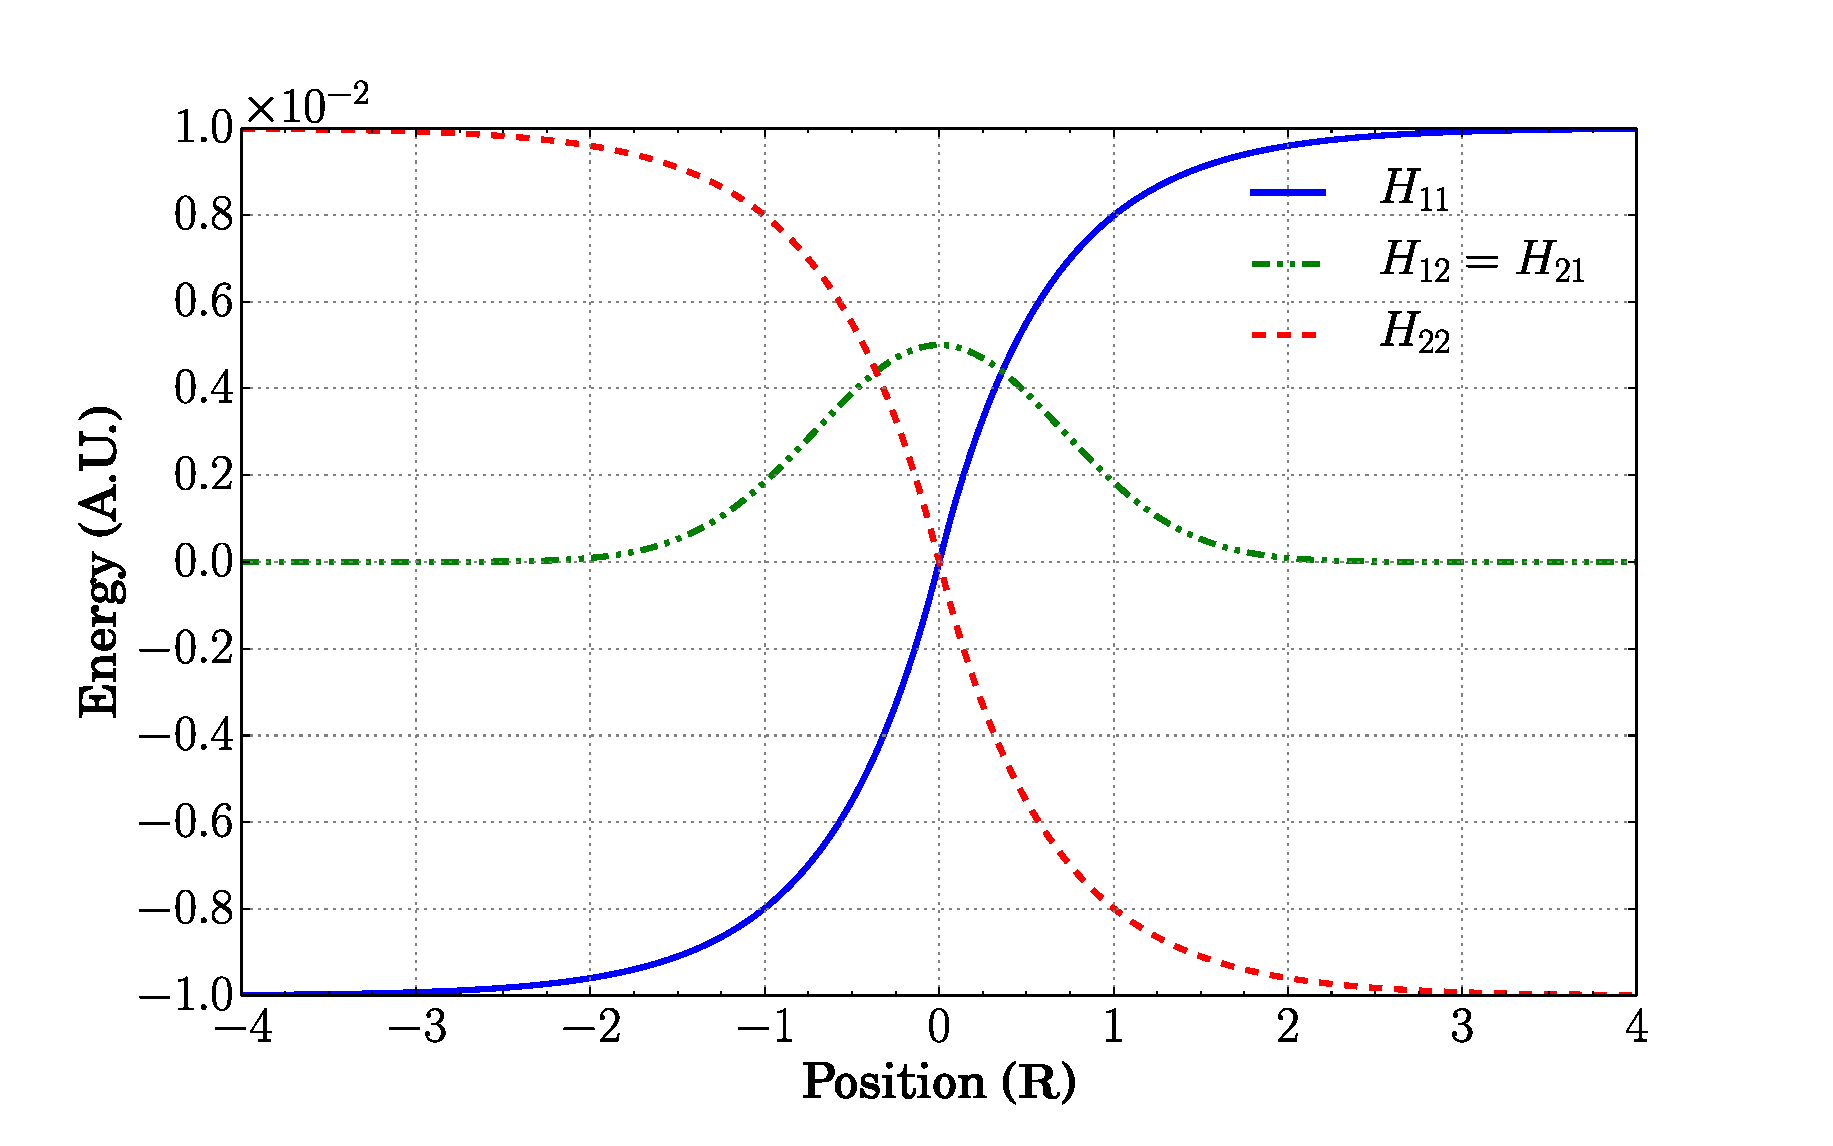
\includegraphics[scale=0.5]{scpes.eps}
\caption[Single avoided crossing: diabatic PES.]{Diabatic PES.}
\label{f:pessc}
\end{figure}

The equations of motion (\cref{eq:diab_motion}) require the calculation of 
gradients for all relevant PES. For our purposes, they can be obtained 
analytically \cref{eq:dscpes}, reducing computational demands. Less ideal 
systems would require numerical differentiation. The diabatic PES derivatives 
are:
\begin{subequations}\label{eq:dscpes}
\begin{align}
\dpar{H_{11}}{R} & = 
A B \begin{cases}
e^{-B R} &\qquad R \geq 0\\
e^{B R} &\qquad R < 0
\end{cases}
\\
\dpar{H_{22}}{R} &= -\dpar{H_{11}}{R}\\
\dpar{H_{12}}{R} &= \dpar{H_{21}}{R} = -2 C D e^{-D R^{2}} R~.
\end{align}
\end{subequations}
They are shown in \cref{f:dpessc}.

\begin{figure}
\centering
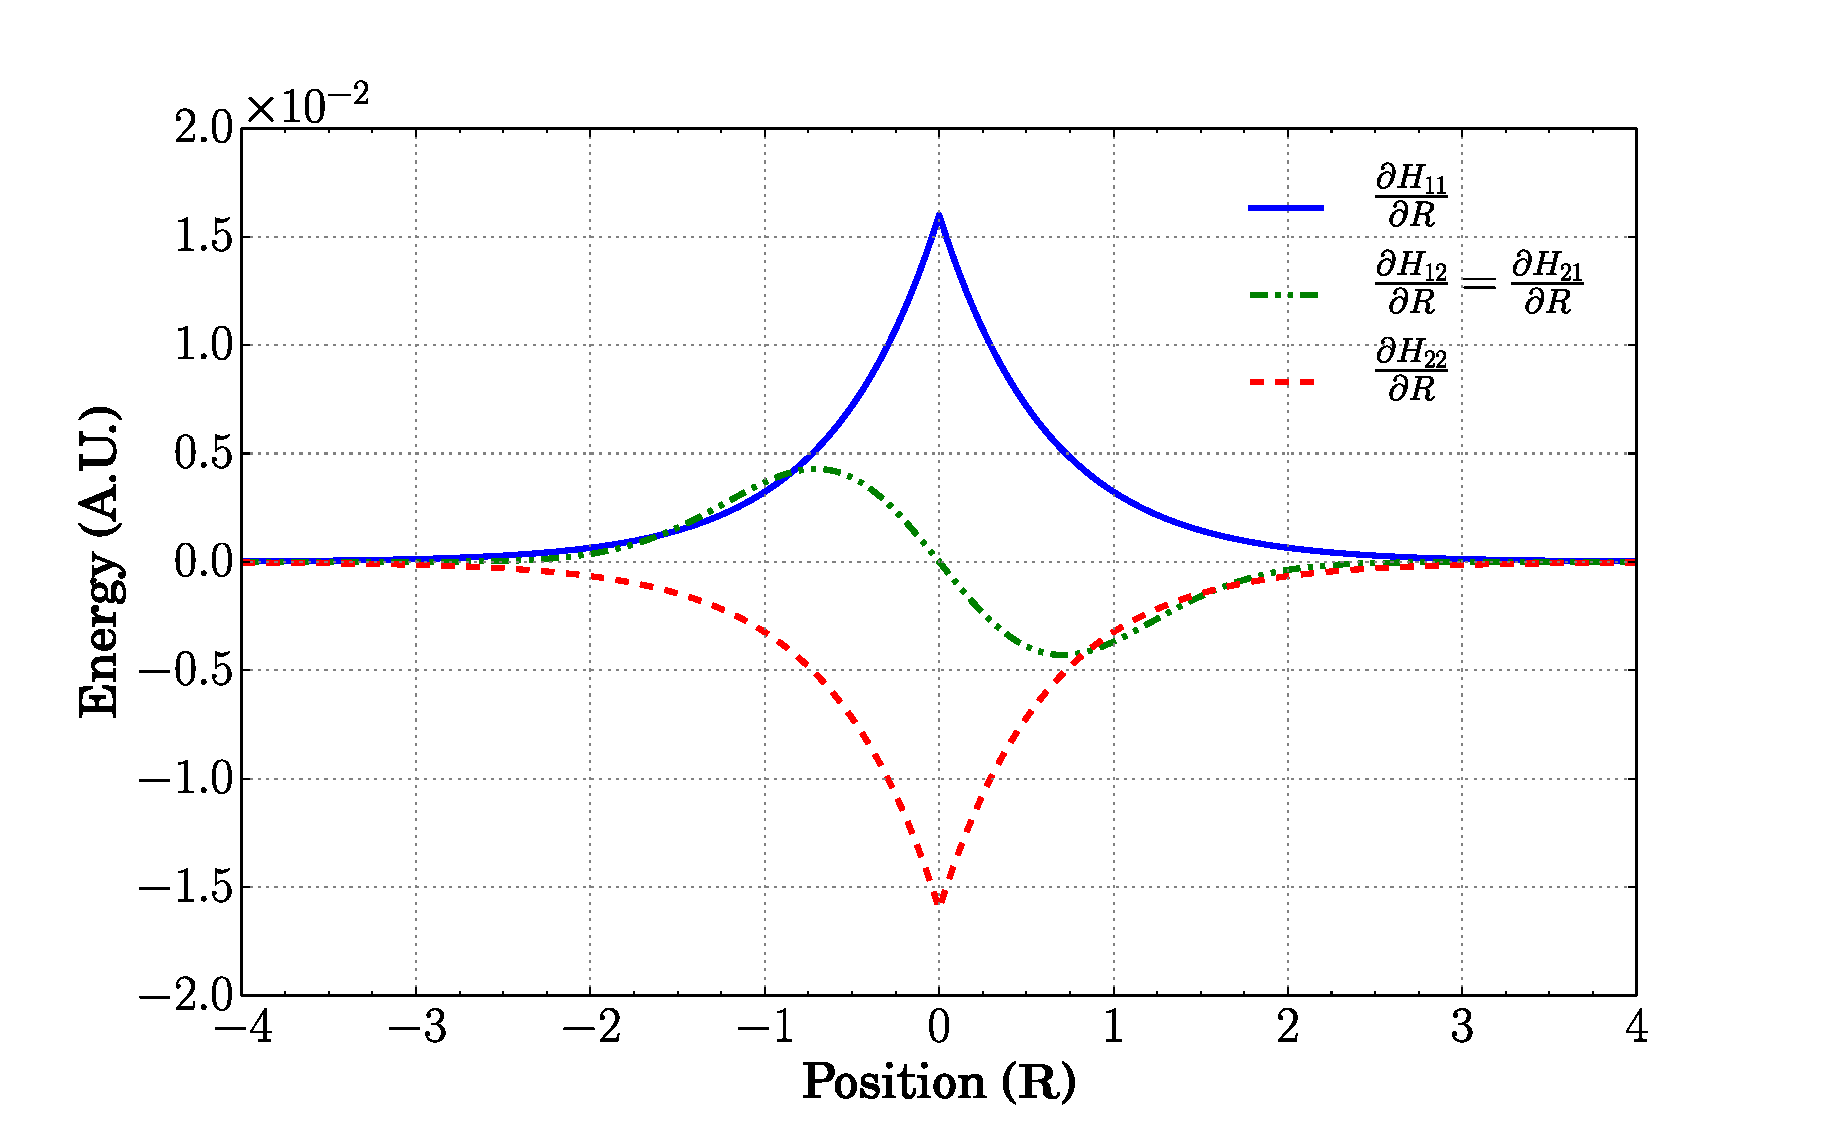
\includegraphics[scale=0.5]{dscpes.eps}
\caption[Single avoided crossing: diabatic PES derivatives.]{Diabatic PES derivatives.}
\label{f:dpessc}
\end{figure}

The adiabatic PES ($ E_{i} $) are the eigenvalues of the diabatic PES 
Hamiltonian matrix, which are obtained through eigenvalue decomposition. In our 
case, they can be obtained analytically, but less ideal systems require 
numerical methods. For the single avoided crossing, these are,
\begin{subequations}\label{eq:ascpes}
\begin{align}
E_{1} &= -e^{-D R^{2}}
\sqrt{
C^{2} + A^{2}e^{2 D R^{2}}
\begin{cases}
\left(1 - e^{-B R}\right)^{2} &\qquad R\geq 0\\
\left(1 - e^{B R}\right)^{2} &\qquad R<0
\end{cases}
}\\
E_{2} & = -E_{1}~.
\end{align}
\end{subequations}
The diabatic Hamiltonian \cref{eq:def_diab_ham} does not require the 
calculation of adiabatic PES, or their derivatives. However, it is often useful 
to visualise the adiabatic PES because they can provide us with useful physical 
insight. They are shown in \cref{f:apessc}. Their derivatives are not shown here because they are irrelevant.

\begin{figure}
\centering
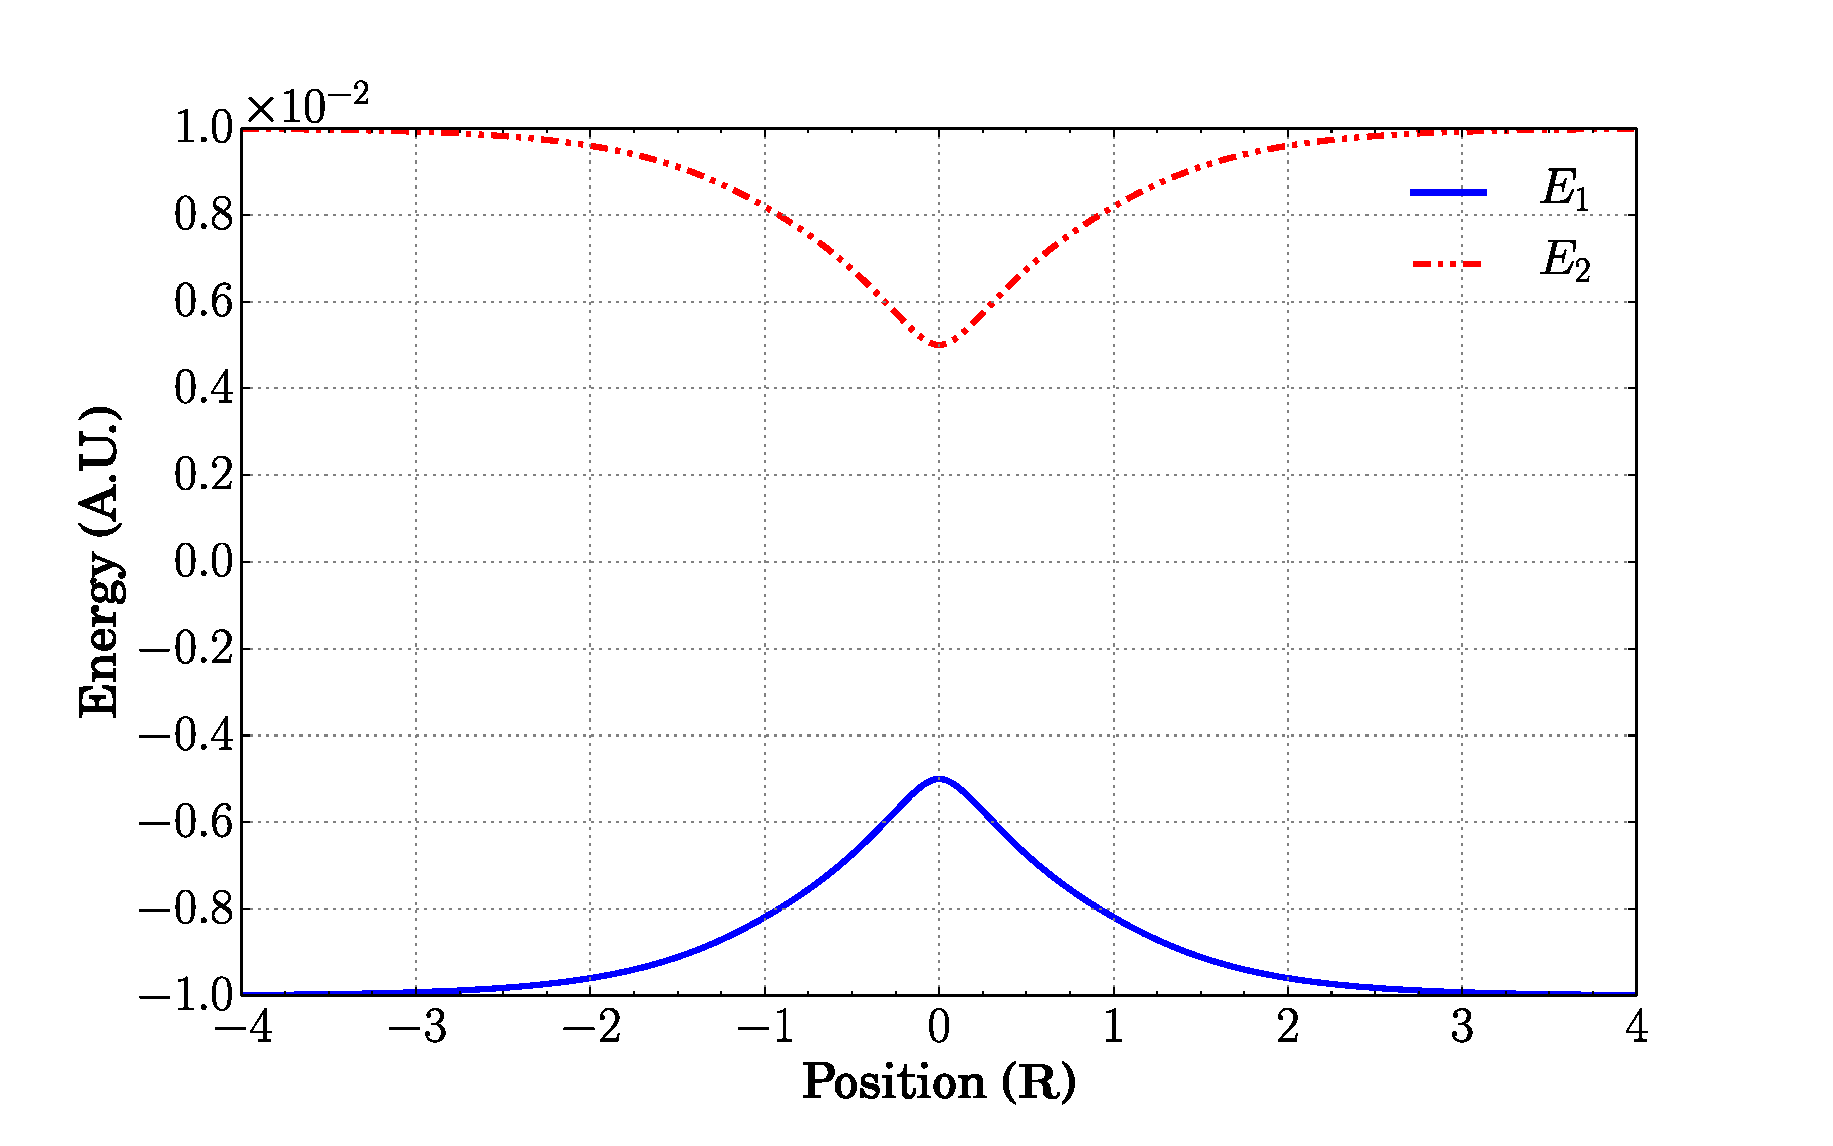
\includegraphics[scale=0.5]{ascpes.eps}
\caption[Single avoided crossing: adiabatic PES.]{Adiabatic PES. Eigenvalues of the diabatic Hamiltonian matrix.}
\label{f:apessc}
\end{figure}

The coupling between electronic states---and therefore the probability of transition---is at its greatest where there the energy difference between both adiabatic PES is at a minimum, as shown in \cref{f:delapessc}.

\begin{figure}
\centering
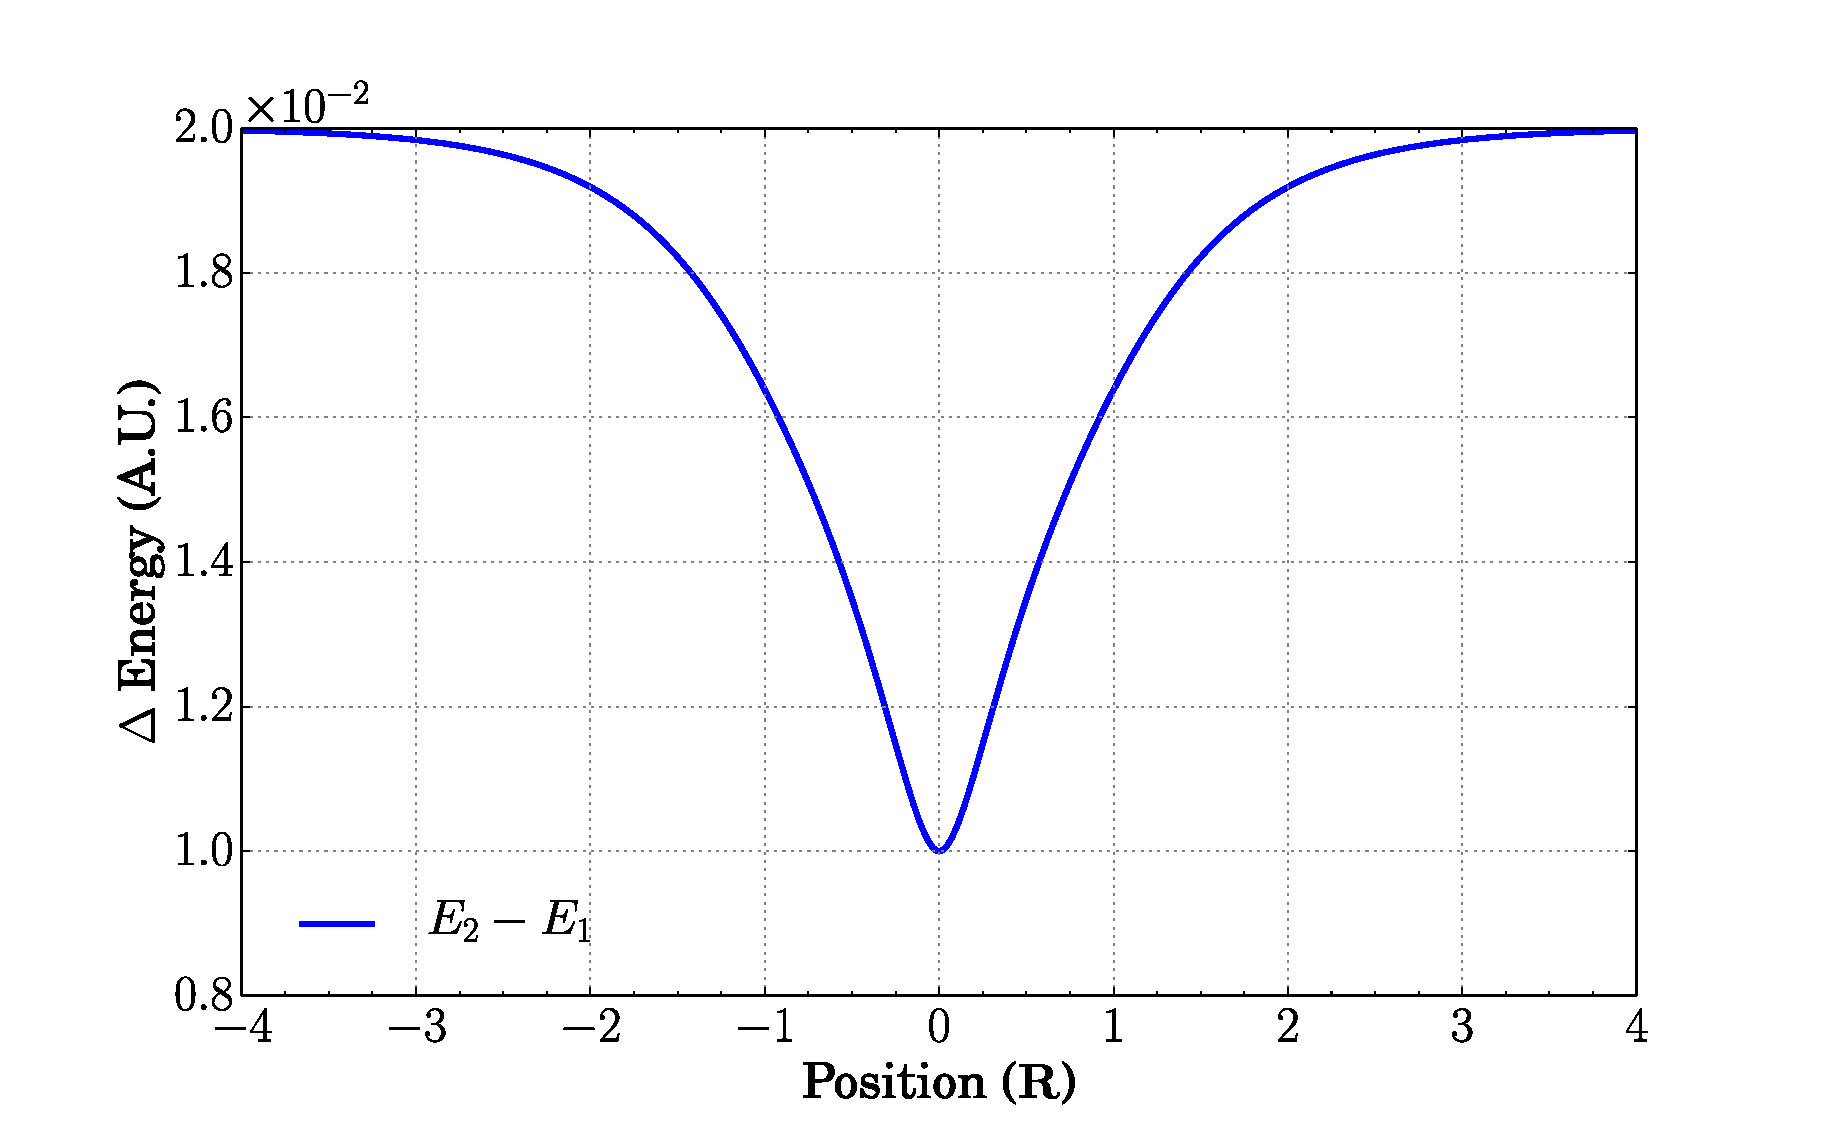
\includegraphics[scale=0.5]{del_ascpes.eps}
\caption[Single avoided crossing: energy difference between adiabatic PES.]{Energy difference between adiabatic PES.}
\label{f:delapessc}
\end{figure}
%
\subsubsection{Equations of Motion}
%
For the single avoided crossing, the equations of motion are:
\begin{subequations}
\begin{align}
\dot{R} & = \frac{P}{\mu}\\
\dot{P} & = 2 C D R e^{-D R^2} (p_{1} p_{2}+ x_{1} x_{2})-\frac{1}{2} \left(p_{1}^{2} + x_{1}^{2} - p_{2}^{2} - x_{2}^{2}\right)
A B \begin{cases}
e^{-B R} &\quad R \geq 0\\
e^{B R} &\quad R < 0
\end{cases}\\
\dot{x}_{1} & = C p_2 e^{-D R^2}+p_1
A \begin{cases}
(1 - e^{-B R}) &\quad R \geq 0\\
(e^{B R} - 1) &\quad R < 0
\end{cases}\\
\dot{p}_{1} & = -C x_2 e^{-D R^2}-x_1
A \begin{cases}
(1 - e^{-B R}) &\quad R \geq 0\\
(e^{B R} - 1) &\quad R < 0
\end{cases}\\
\dot{x}_{2} & = C p_1 e^{-D R^2}-p_2
A \begin{cases}
(1 - e^{-B R}) &\quad R \geq 0\\
(e^{B R} - 1) &\quad R < 0
\end{cases}\\
\dot{p}_{2} & = -C x_1 e^{-D R^2} + x_2
A \begin{cases}
(1 - e^{-B R}) &\quad R \geq 0\\
(e^{B R} - 1) &\quad R < 0
\end{cases}~.
\end{align}
\end{subequations}
%
\subsection{Double Avoided Crossing}\label{s:dac}
%
\subsubsection{Potential Energy Surfaces}
%
The diabatic PES for the double avoided crossing were defined by Tully \cite{tully} as:
\begin{subequations}
\begin{align}
H_{11}(R) &= 0 \\
H_{22}(R) &= -A e^{-B R^{2}} + E_{0}\\
H_{12}(R) &= H_{21}(R) = C e^{-D R^{2}}~,
\end{align}
\end{subequations}
where $ A = 0.1,~B = 0.28,~C = 0.015,~D = 0.06,~\text{and}~E_{0} = 0.05$. They are shown in \cref{f:pesdc}.

\begin{figure}
\centering
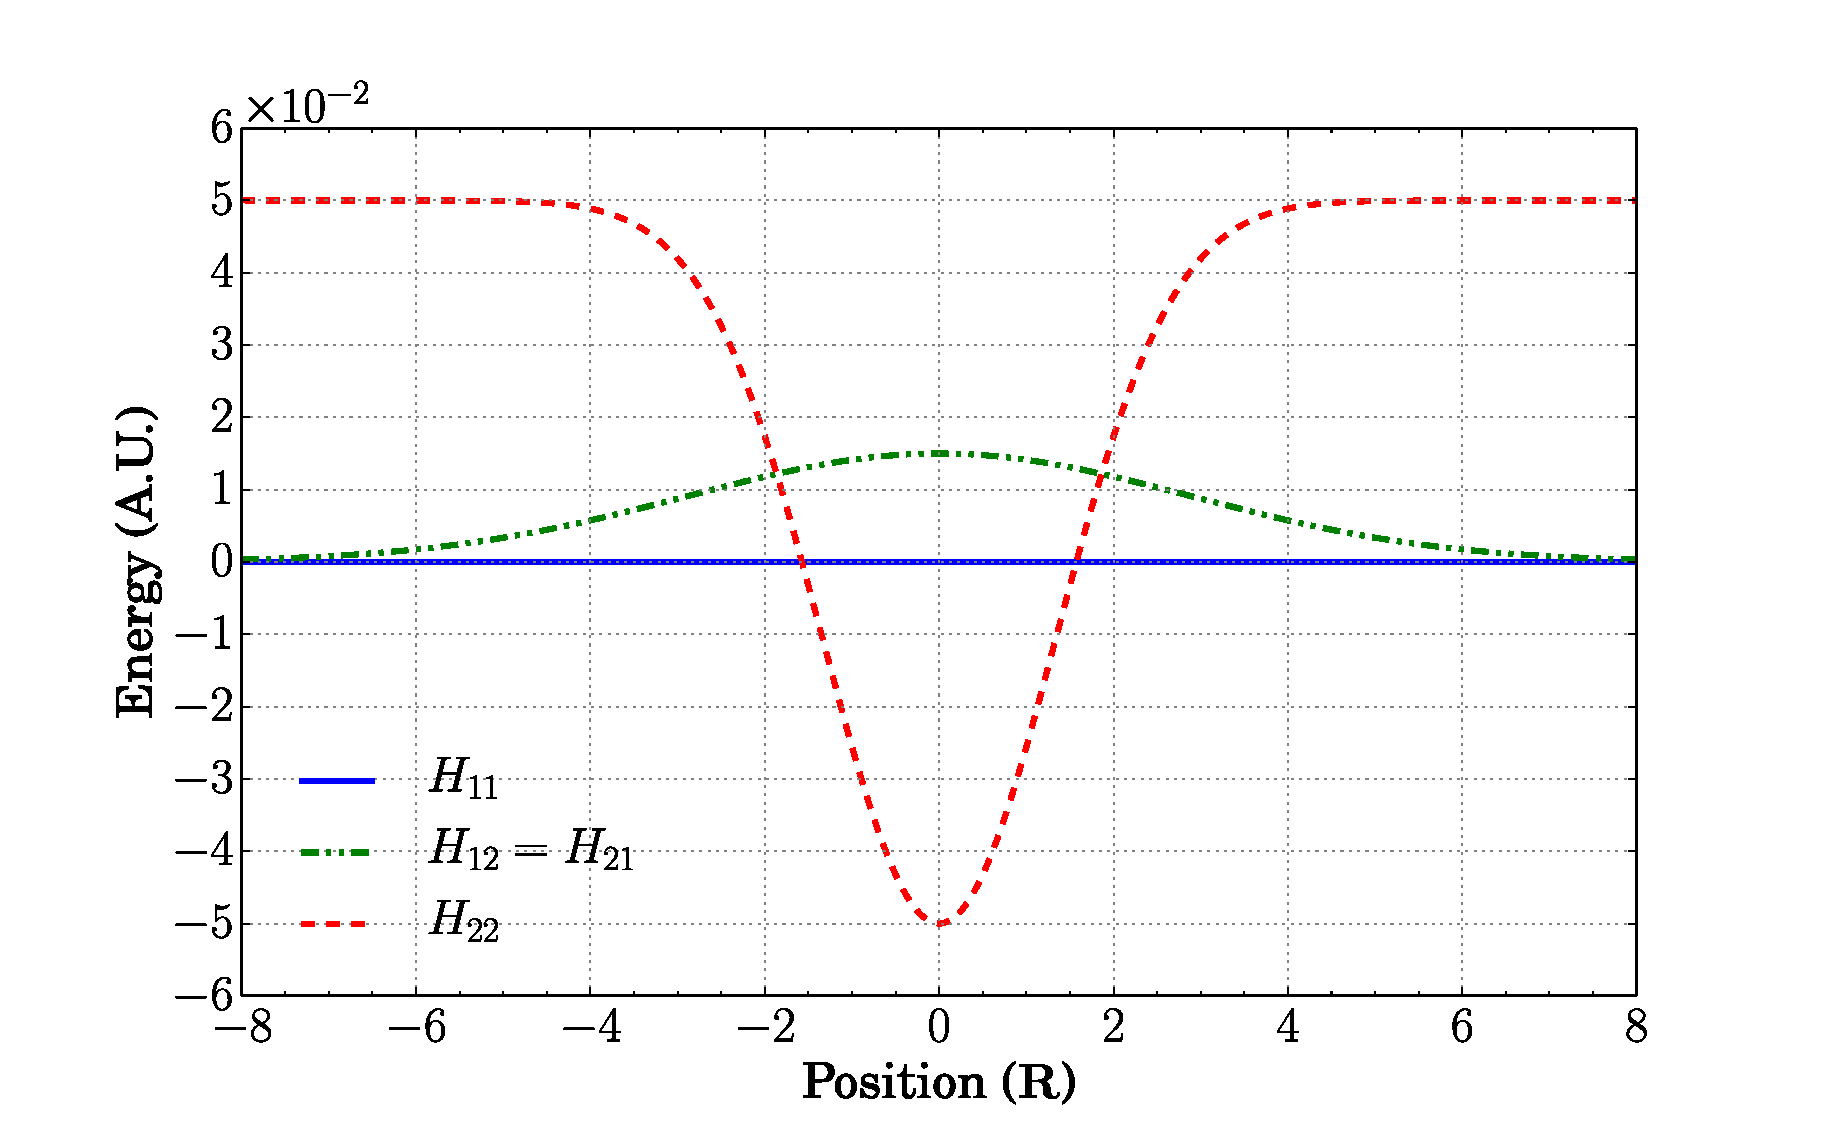
\includegraphics[scale=0.5]{dcpes.eps}
\caption[Double avoided crossing: diabatic PES.]{Diabatic PES.}
\label{f:pesdc}
\end{figure}

Their derivatives are:
\begin{subequations}
\begin{align}
\dpar{H_{11}}{R} &= 0\\
\dpar{H_{22}}{R} &= 2 A B e^{-B R^{2}} R\\
\dpar{H_{12}}{R} &= \dpar{H_{21}}{R} = -2 C D e^{-D R^{2}} R~.
\end{align}
\end{subequations}
They are shown in \cref{f:dpesdc}.

\begin{figure}
\centering
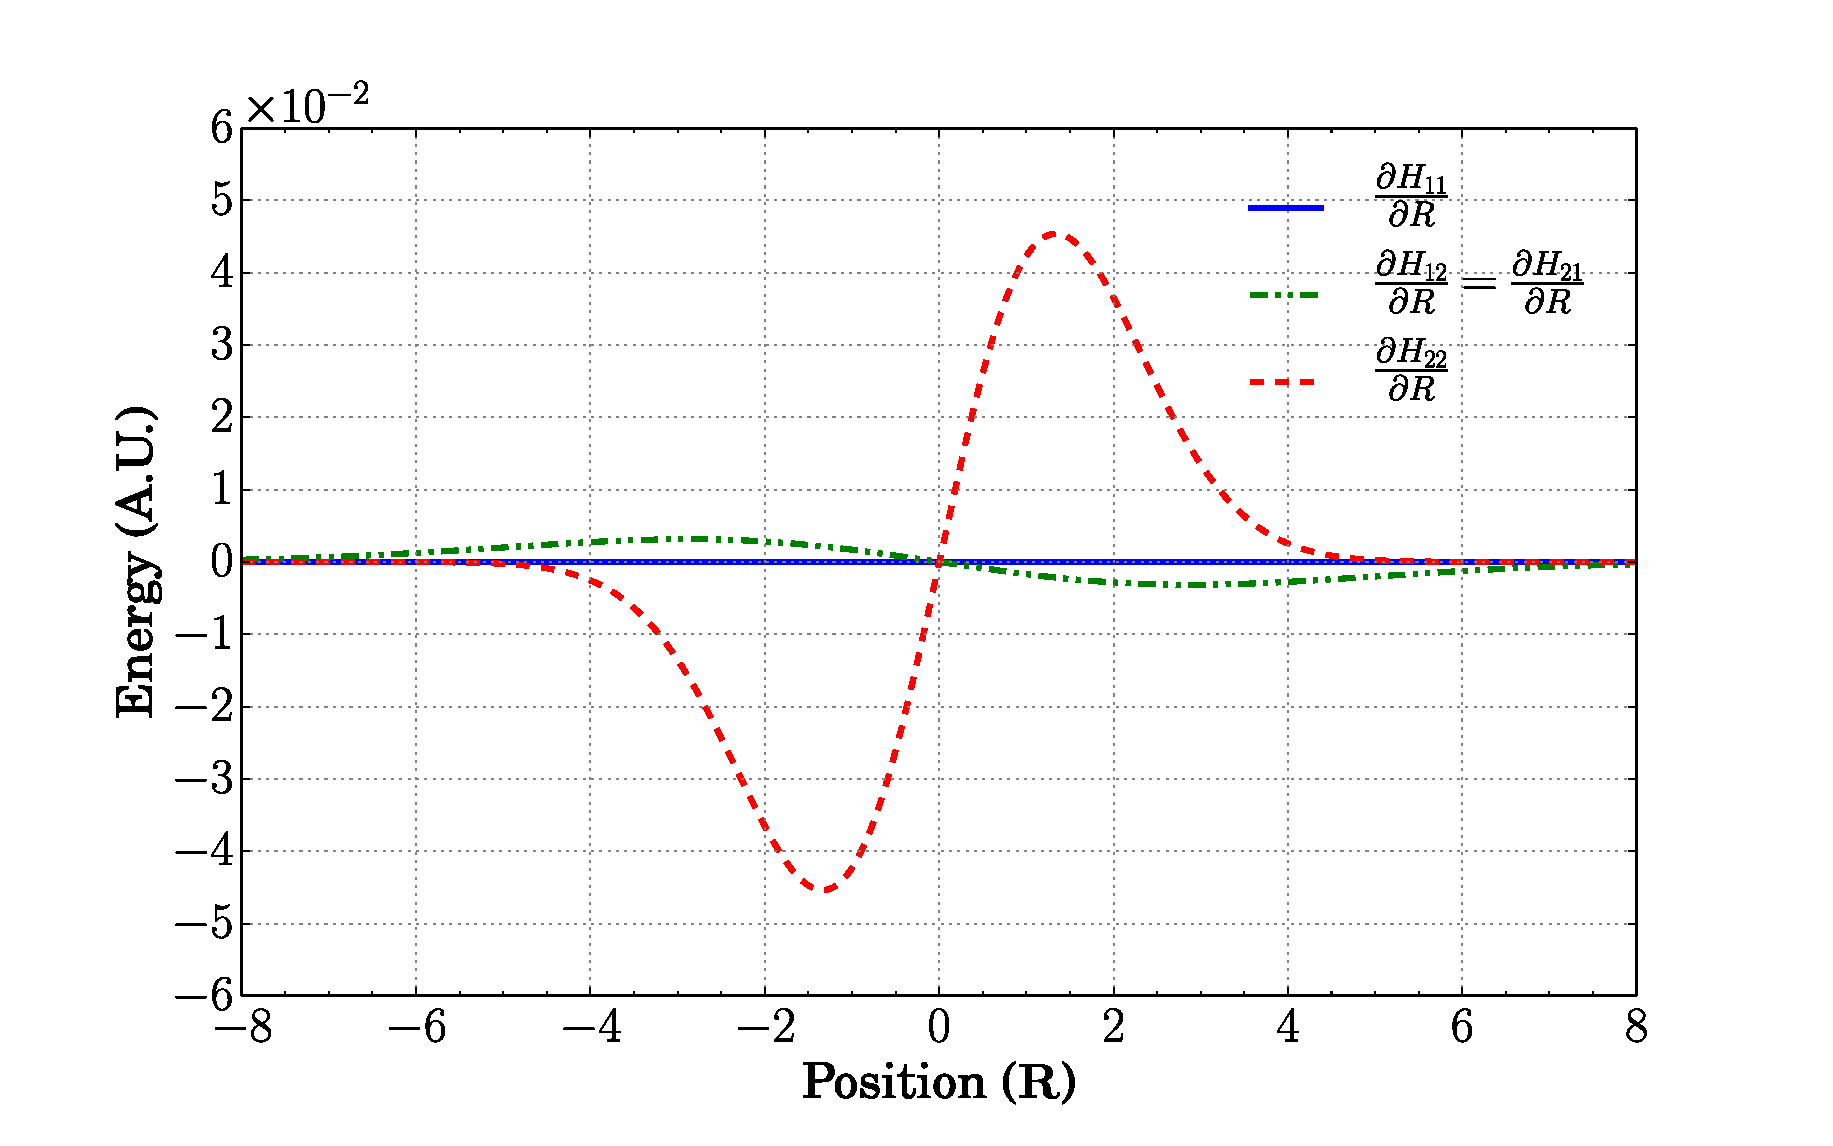
\includegraphics[scale=0.5]{ddcpes.eps}
\caption[Double avoided crossing: diabatic PES derivatives.]{Diabatic PES derivatives.}
\label{f:dpesdc}
\end{figure}

The adiabatic PES are:
\begin{subequations}
\begin{align}
E_{1} &= \frac{1}{2} e^{-(B+D) R^{2}}
\left(
-A e^{D R^{2}} + e^{(B+D) R^{2}} E_{0} -
\sqrt{
4 C^{2} e^{2 B R^{2}} + e^{2 D R^{2}}\left( A - e^{B R^{2}} E_{0} \right)^{2}
}
\right)\\
E_{2} &= \frac{1}{2} e^{-(B+D) R^{2}}
\left(
-A e^{D R^{2}} + e^{(B+D) R^{2}} E_{0} +
\sqrt{
4 C^{2} e^{2 B R^{2}} + e^{2 D R^{2}}\left( A - e^{B R^{2}} E_{0} \right)^{2}
}
\right)~.
\end{align}
\end{subequations}
They are shown in \cref{f:apesdc}

\begin{figure}
\centering
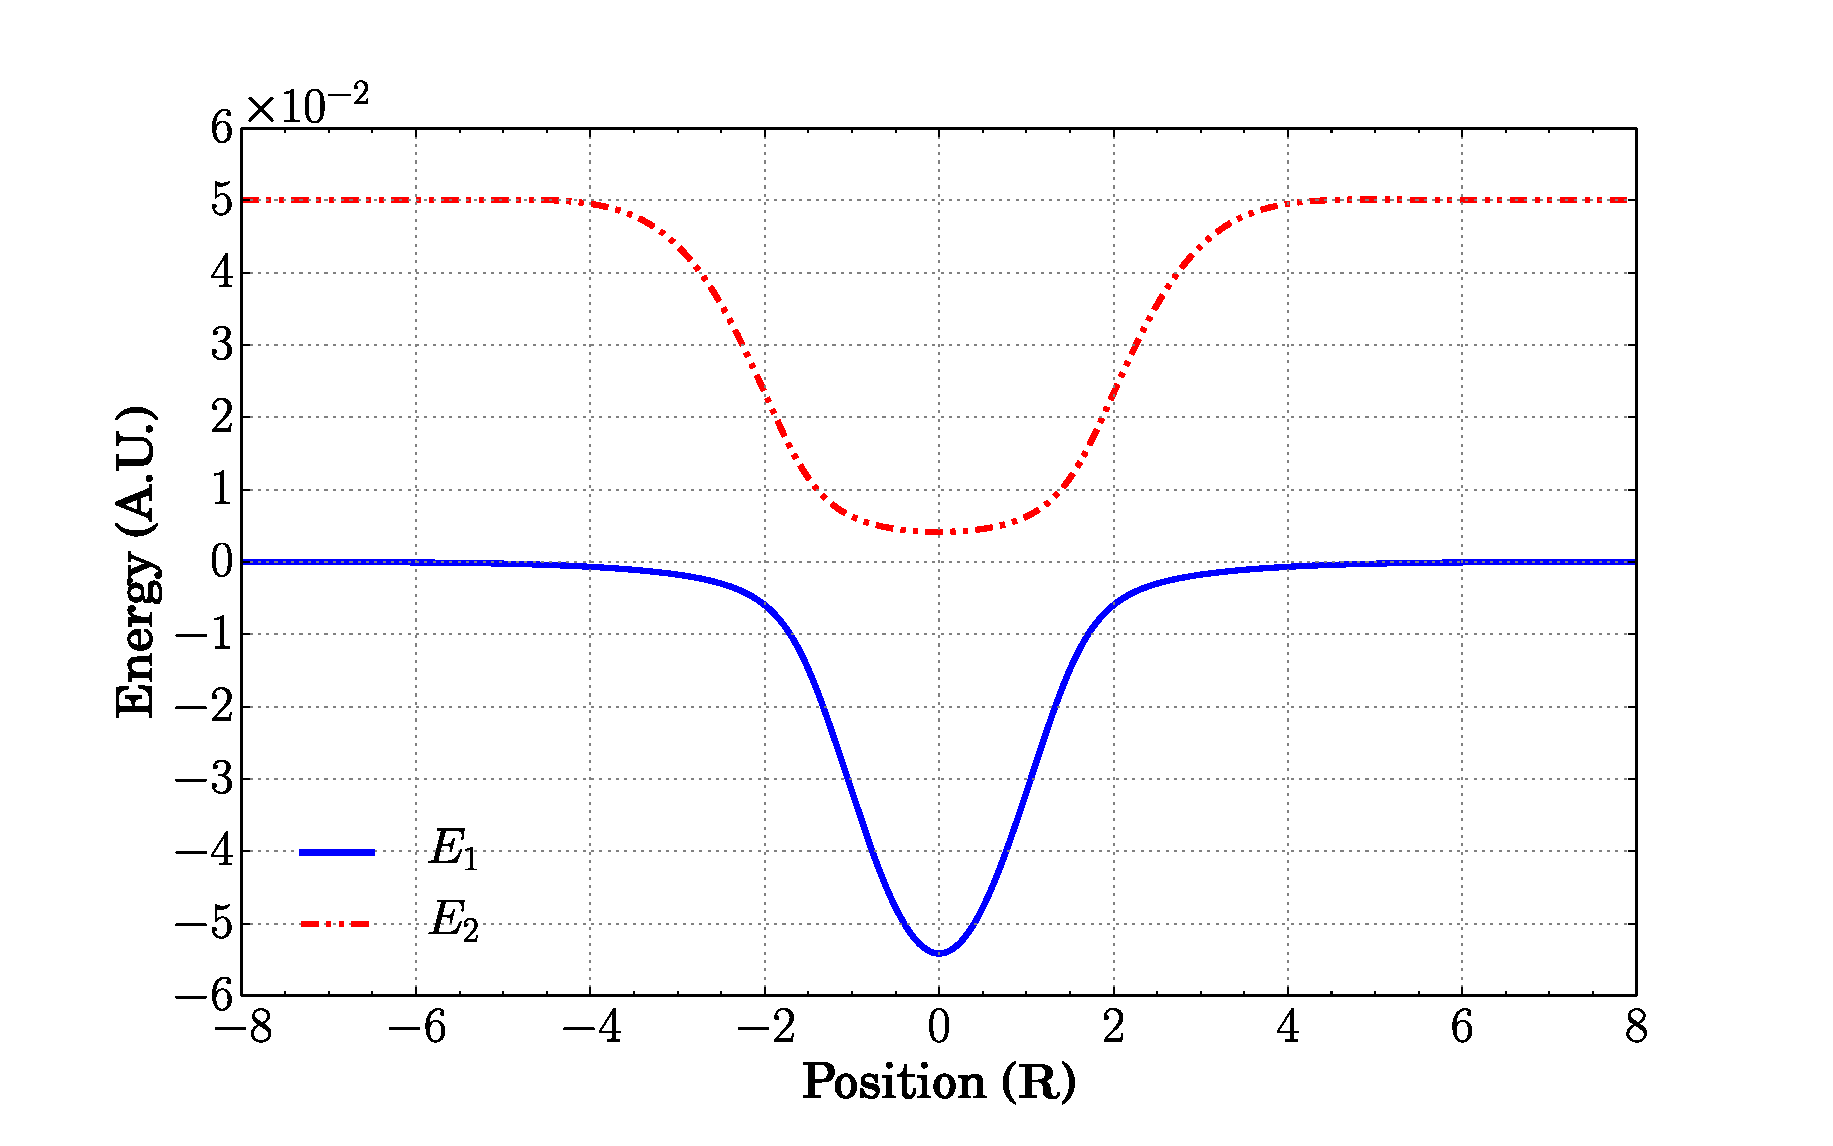
\includegraphics[scale=0.5]{adcpes.eps}
\caption[Double avoided crossing: adiabatic PES.]{Adiabatic PES. Eigenvalues of the diabatic Hamiltonian matrix.}
\label{f:apesdc}
\end{figure}

In this case, there are two minimum energy gaps between both adiabatic PES, shown in \cref{f:delapesdc}. This brings about some rather interesting behaviours shown in \cref{s:rdac}.

\begin{figure}
\centering
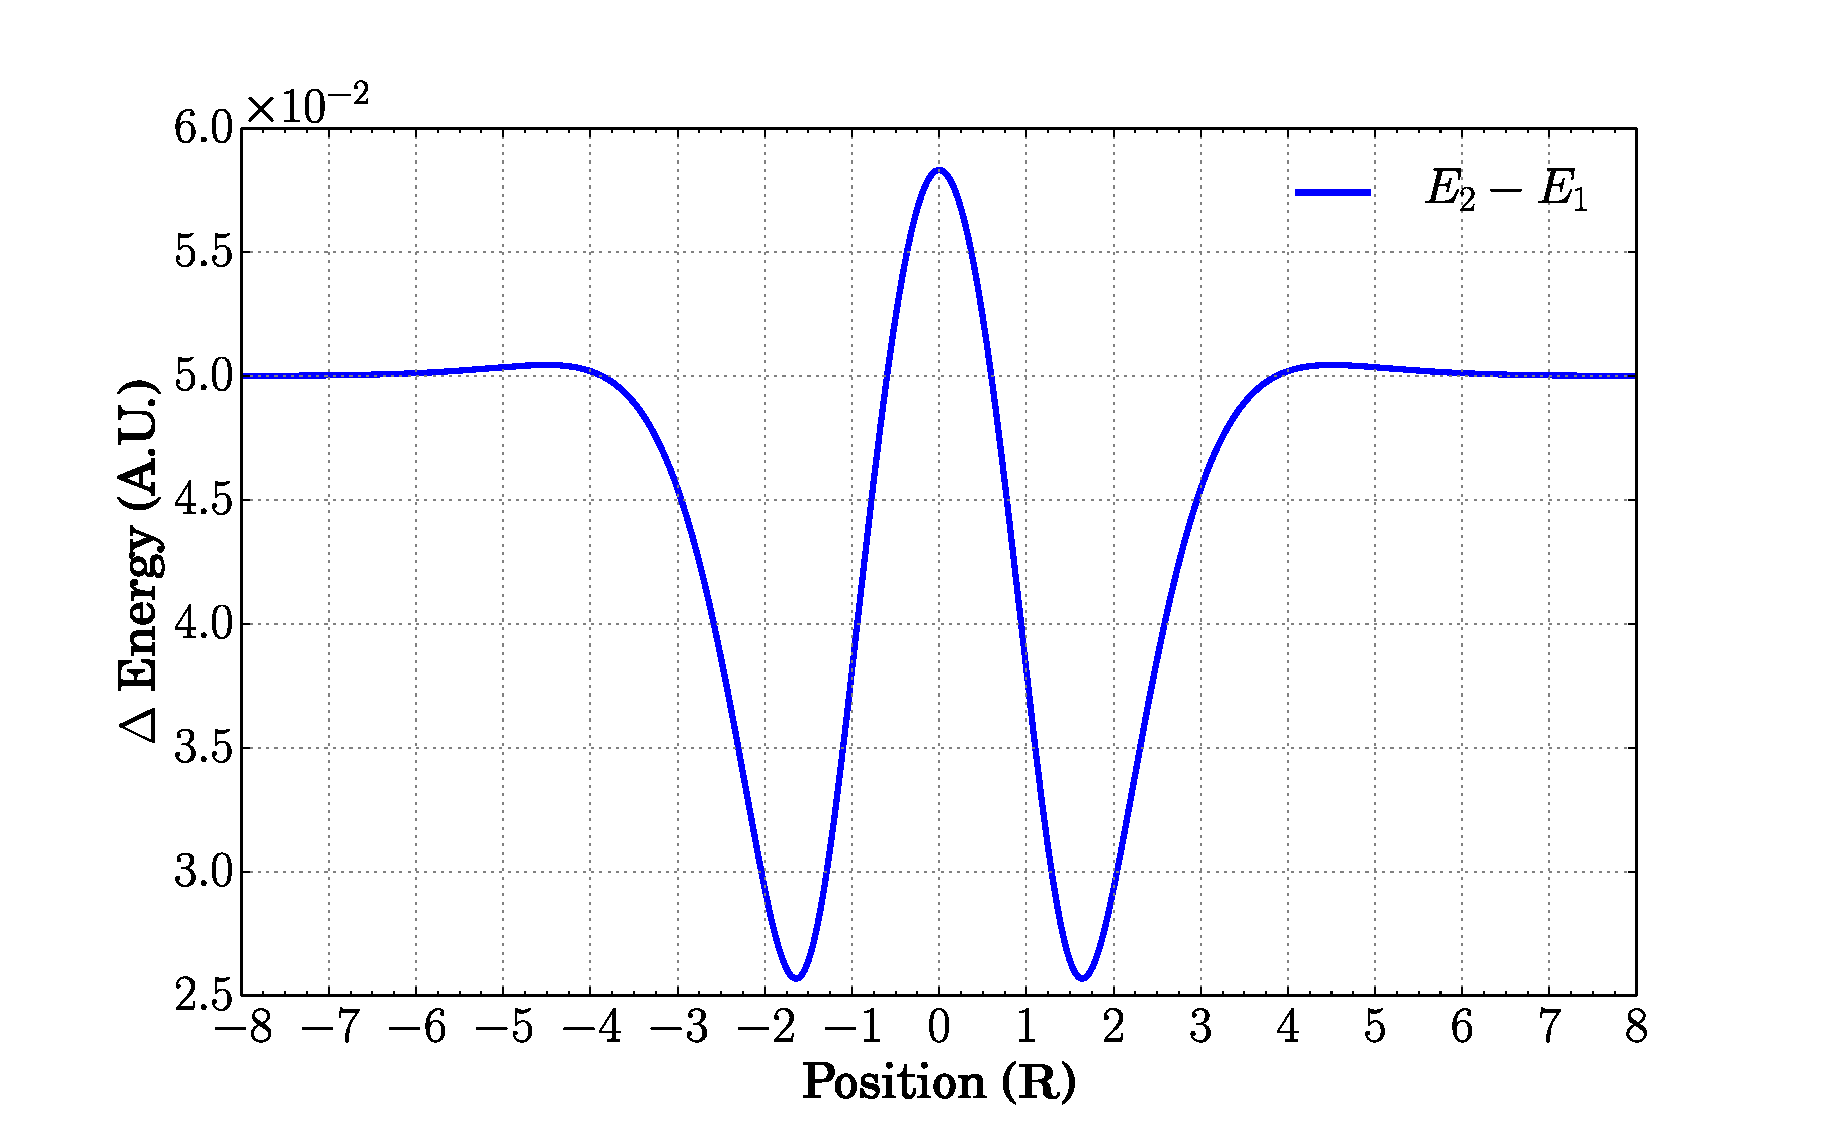
\includegraphics[scale=0.5]{del_adcpes.eps}
\caption[Double avoided crossing: energy difference between adiabatic PES.]{Energy difference between adiabatic PES.}
\label{f:delapesdc}
\end{figure}
%
\subsubsection{Equations of Motion}
%
For the double avoided crossing, the equations of motion are:
\begin{subequations}
\begin{align}
\dot{R} & = \frac{P}{\mu }\\
\dot{P} & = R \left(A B e^{-B R^2} \left(\frac{p_1^2}{2}-\frac{p_2^2}{2}+\frac{x_1^2}{2}-\frac{x_2^2}{2}-1\right)+2 C D e^{-D R^2} (p_1 p_2+ x_1 x_2)\right)\\
\dot{x}_{1} & = \frac{1}{2} p_1 \left(A e^{-B R^2}-E_0\right)+C p_2 e^{-D R^2}\\
\dot{p}_{1} & = -\frac{1}{2} x_1 \left(A e^{-B R^2}-E_0\right)-C x_2 e^{-D R^2}\\
\dot{x}_{2} & = -\frac{1}{2} p_2 \left(A e^{-B R^2}-E_0\right) + C p_1 e^{-D R^2}\\
\dot{p}_{2} & = \frac{1}{2} x_2 \left(A e^{-B R^2}-E_0\right)-C x_1 e^{-D R^2}~.
\end{align}
\end{subequations}
%
\subsection{Extended Coupling}\label{s:ec}
%
\subsubsection{Potential Energy Surfaces}
%
This problem has non-vanishing non-diagonal elements in the Hamiltonian matrix. Said elements are perturbations from a pure state, and when they do not vanish as $ R \rightarrow \pm\infty $, one must use the adiabatic Hamiltonian. The diagonal elements of the Hamiltonian matrix are also constant, lending further arguments to the use of the adiabatic Hamiltonian due to the system's relatively unchanging conditions.

The diabatic PES for the extended coupling problem were defined by Tully \cite{tully} as:
\begin{subequations}
\begin{align}
H_{11}(R) & = -A\\
H_{22}(R) & = -H_{11}\\
H_{12}(R) & = H_{21}(R) = 
B\begin{cases}
\left(2 - e^{-C R}\right) &\qquad R \geq 0 \\
e^{C R} &\qquad R<0
\end{cases}~,
\end{align}
\end{subequations}
where $ A = 6 \times 10^{-4},~B = 0.1,~\text{and}~C = 0.9$. They are shown in \cref{f:pesec}.

\begin{figure}
\centering
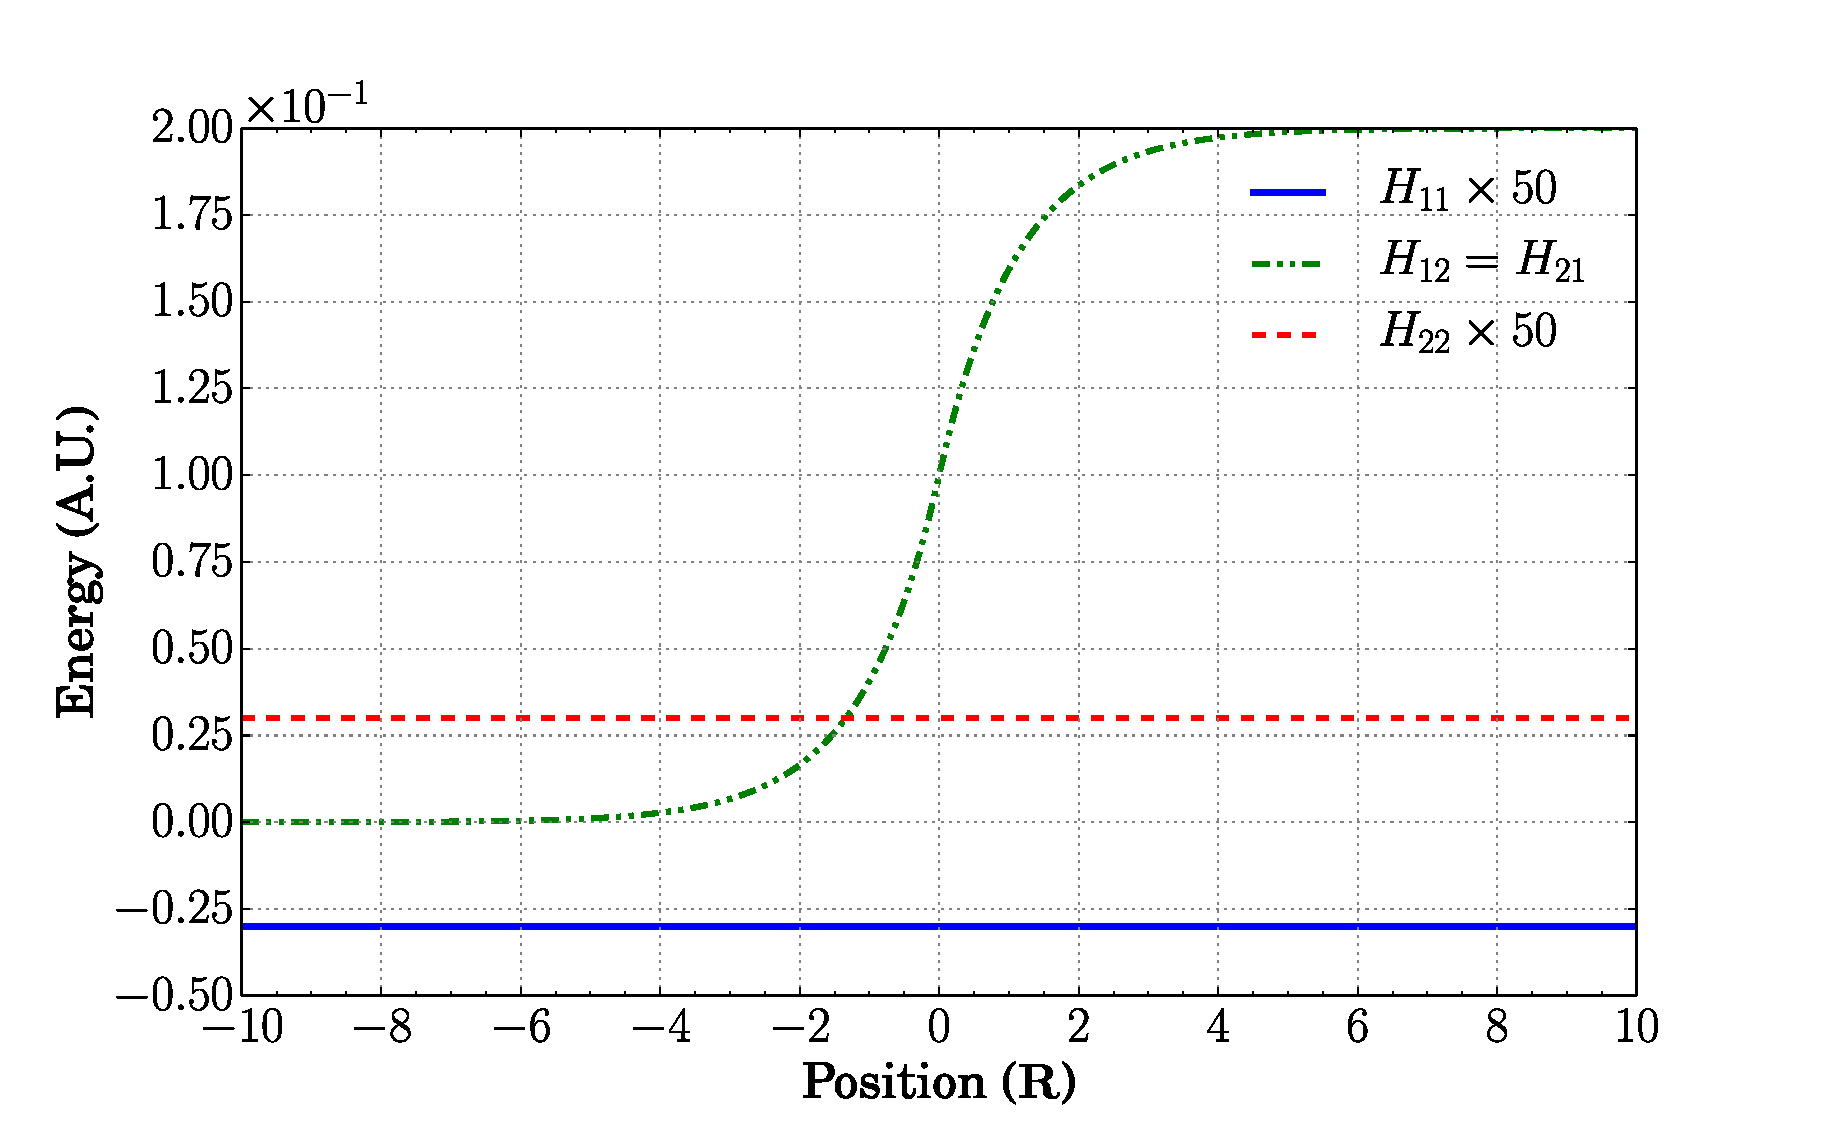
\includegraphics[scale=0.5]{ecpes.eps}
\caption[Extended coupling: diabatic PES.]{Diabatic PES.}
\label{f:pesec}
\end{figure}

The diabatic PES derivatives are:
\begin{subequations}
\begin{align}
\dpar{H_{11}}{R} &= \dpar{H_{22}}{R} = 0\\
\dpar{H_{12}}{R} &= \dpar{H_{21}}{R} = 
B C\begin{cases}
e^{-C R} &\qquad R \geq 0\\
e^{C R} &\qquad R<0~.
\end{cases}
\end{align}
\end{subequations}
They are shown in \cref{f:dpesec}.

\begin{figure}
\centering
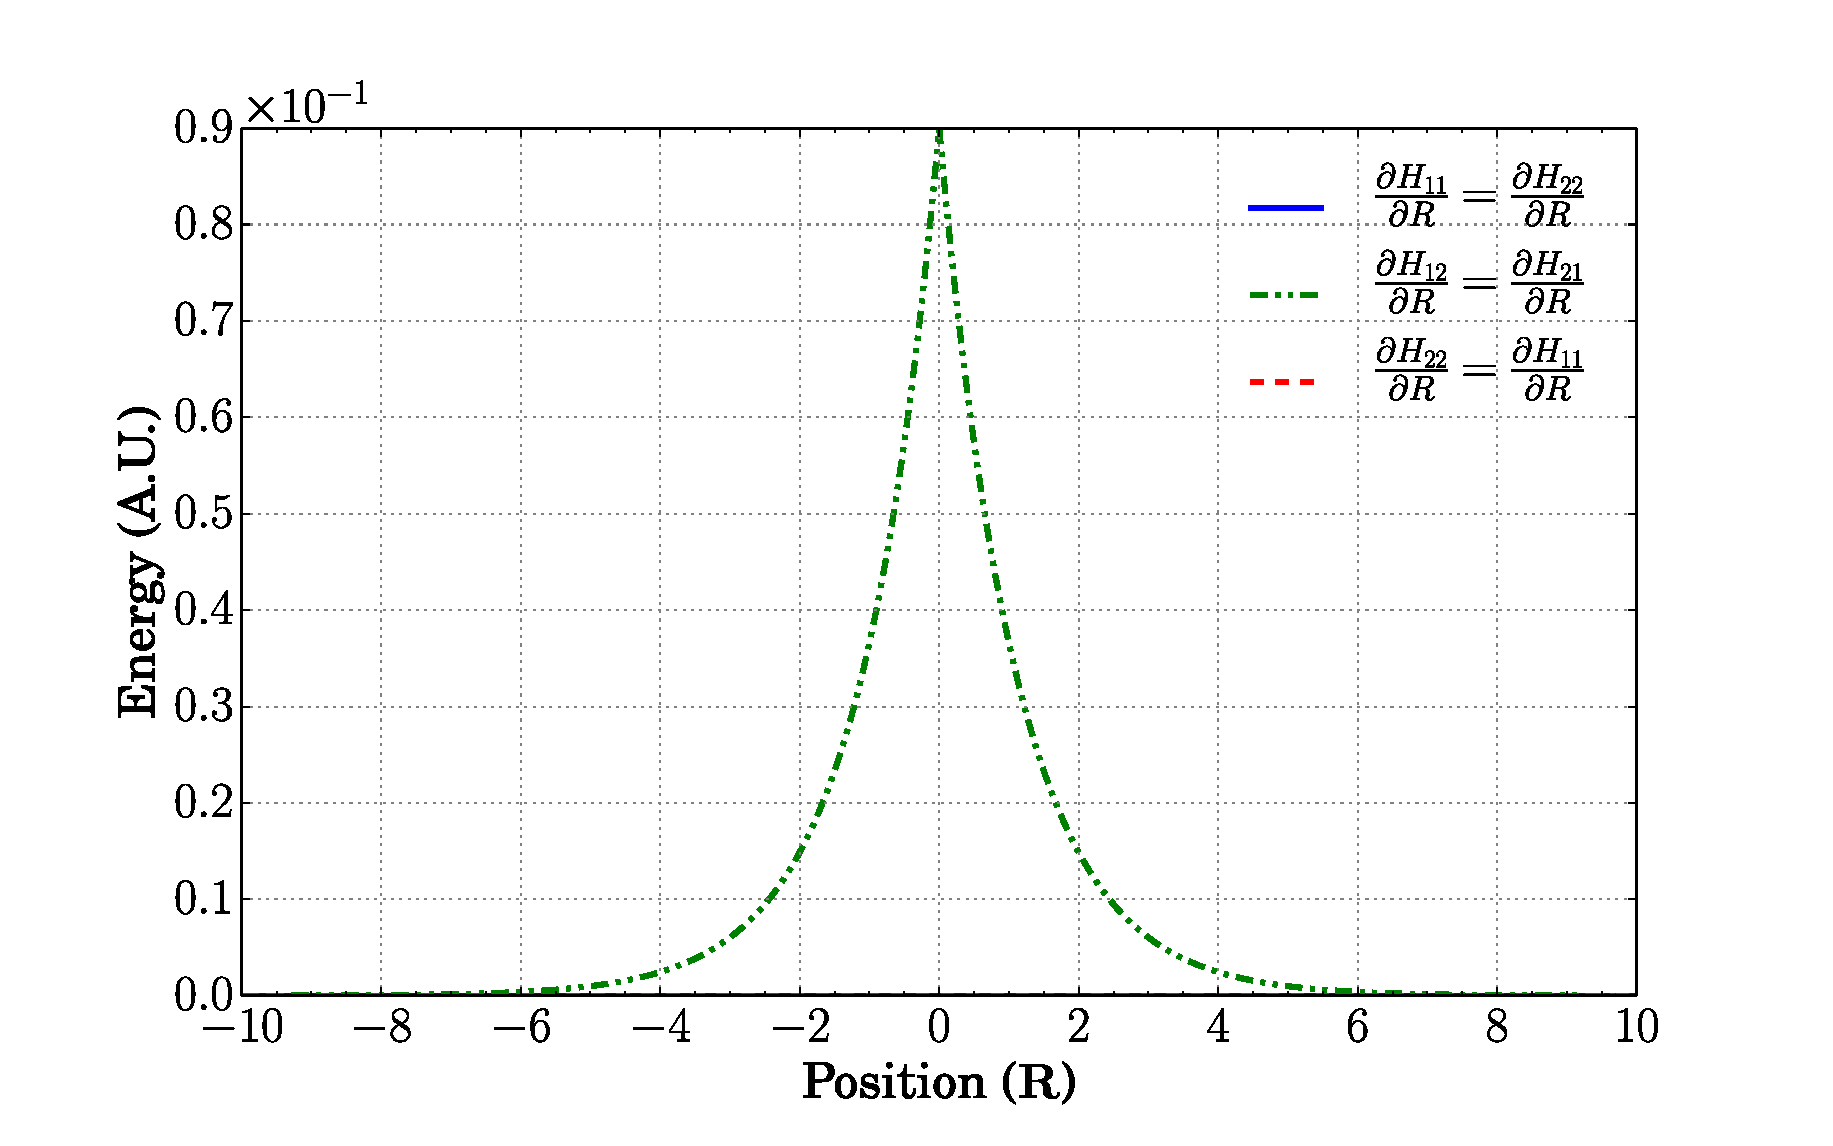
\includegraphics[scale=0.5]{decpes.eps}
\caption[Extended coupling: diabatic PES derivatives.]{Diabatic PES derivatives.}
\label{f:dpesec}
\end{figure}

The adiabatic PES are:
\begin{subequations}
\begin{align}
E_{1} & = -\sqrt{A^{2} 
+ B^{2}\begin{cases}
(2 - e^{-C R})^{2} &\qquad R \geq 0\\
e^{2C R} &\qquad R<0
\end{cases}
}\\
E_{2} &= -E_{1}~.
\end{align}
\end{subequations}
They are shown in \cref{f:apesec}.

\begin{figure}
\centering
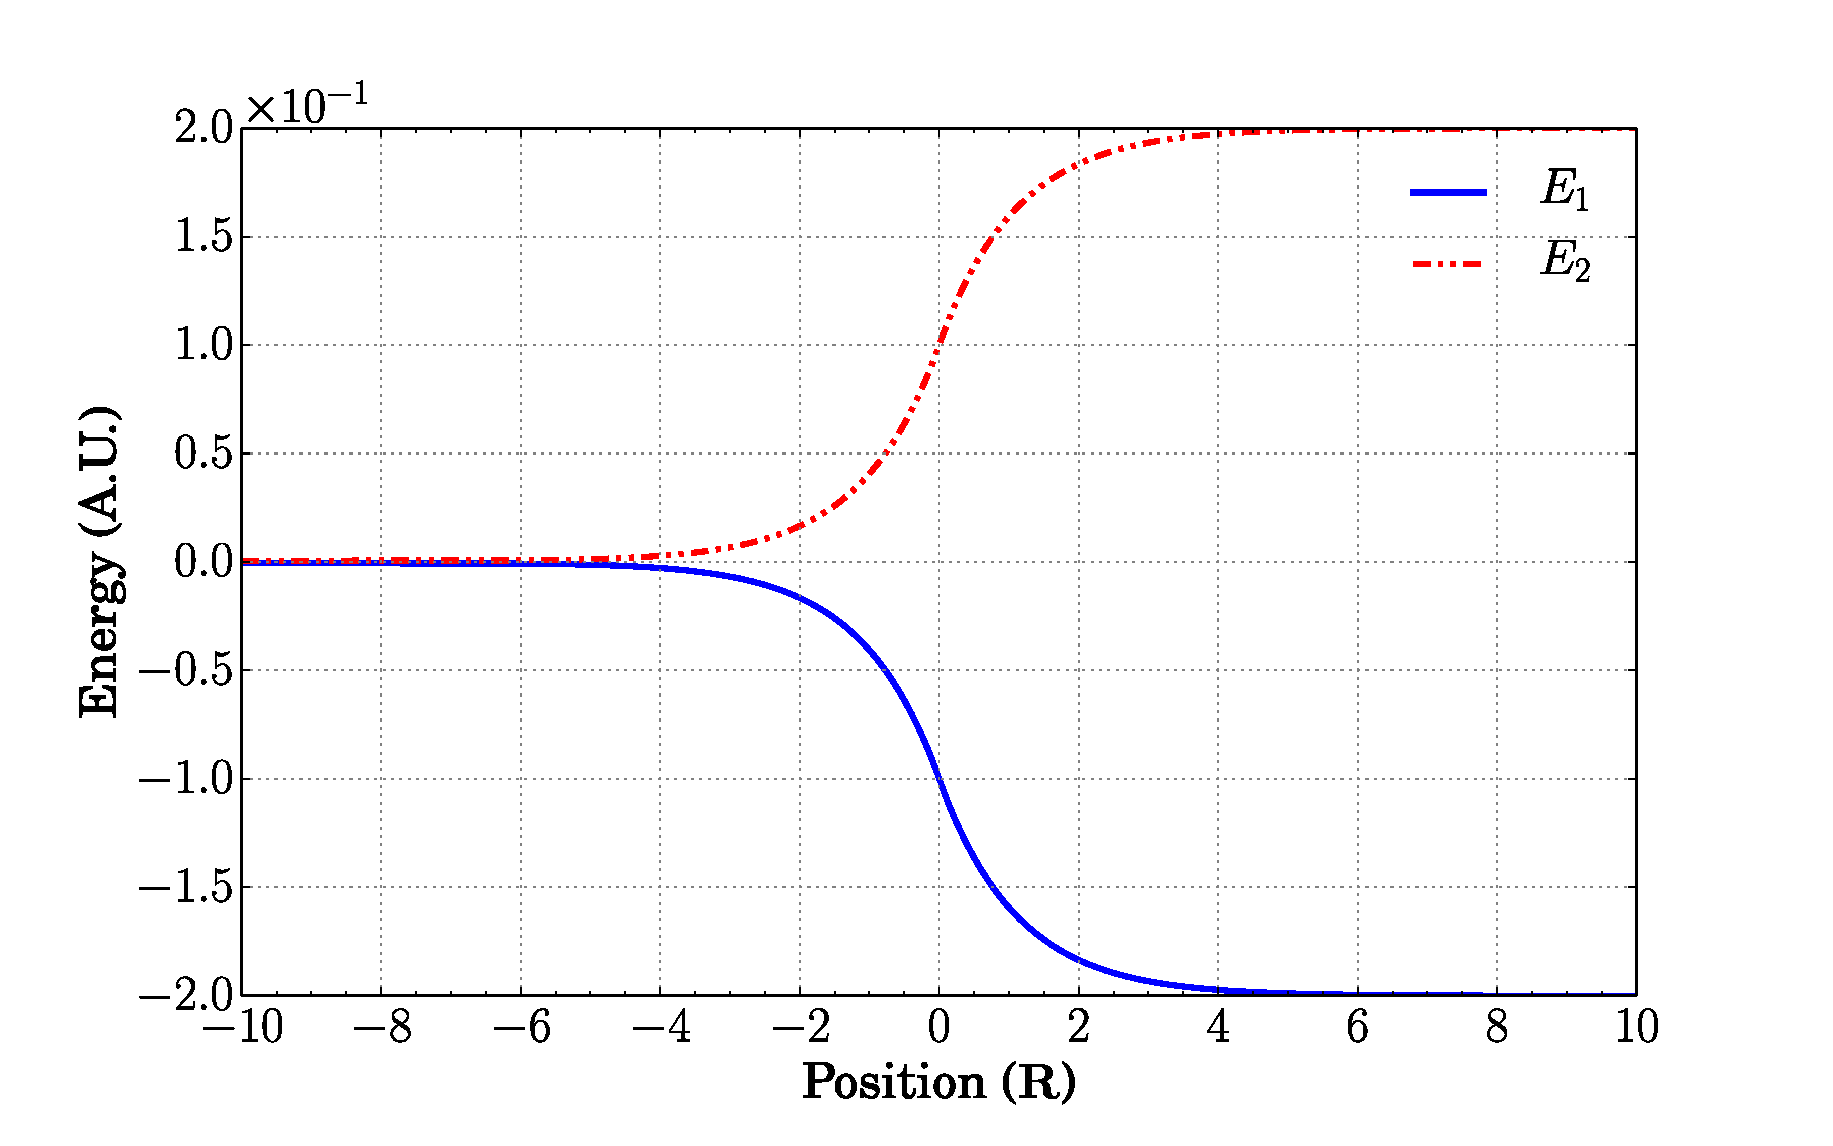
\includegraphics[scale=0.5]{aecpes.eps}
\caption[Extended coupling: adiabatic PES.]{Adiabatic PES. Eigenvalues of the diabatic Hamiltonian matrix.}
\label{f:apesec}
\end{figure}

Their derivatives are:
\begin{subequations}
\begin{align}
\dpar{E_{1}}{R} &=
\begin{cases}
-\dfrac{B^2 C e^{-2 C R} \left(2 e^{C R}-1\right)}{\sqrt{A^2+B^2 \left(e^{-C R}-2\right)^2}} & \qquad R \geq 0\\
-\dfrac{B^2 C e^{2 C R}}{\sqrt{A^2+B^2 e^{2 C R}}} &\qquad R<0
\end{cases}\\
\dpar{E_{2}}{R} &= -\dpar{E_{1}}{R}~.
\end{align}
\end{subequations}
They are shown in \cref{f:dapesec}.

\begin{figure}
\centering
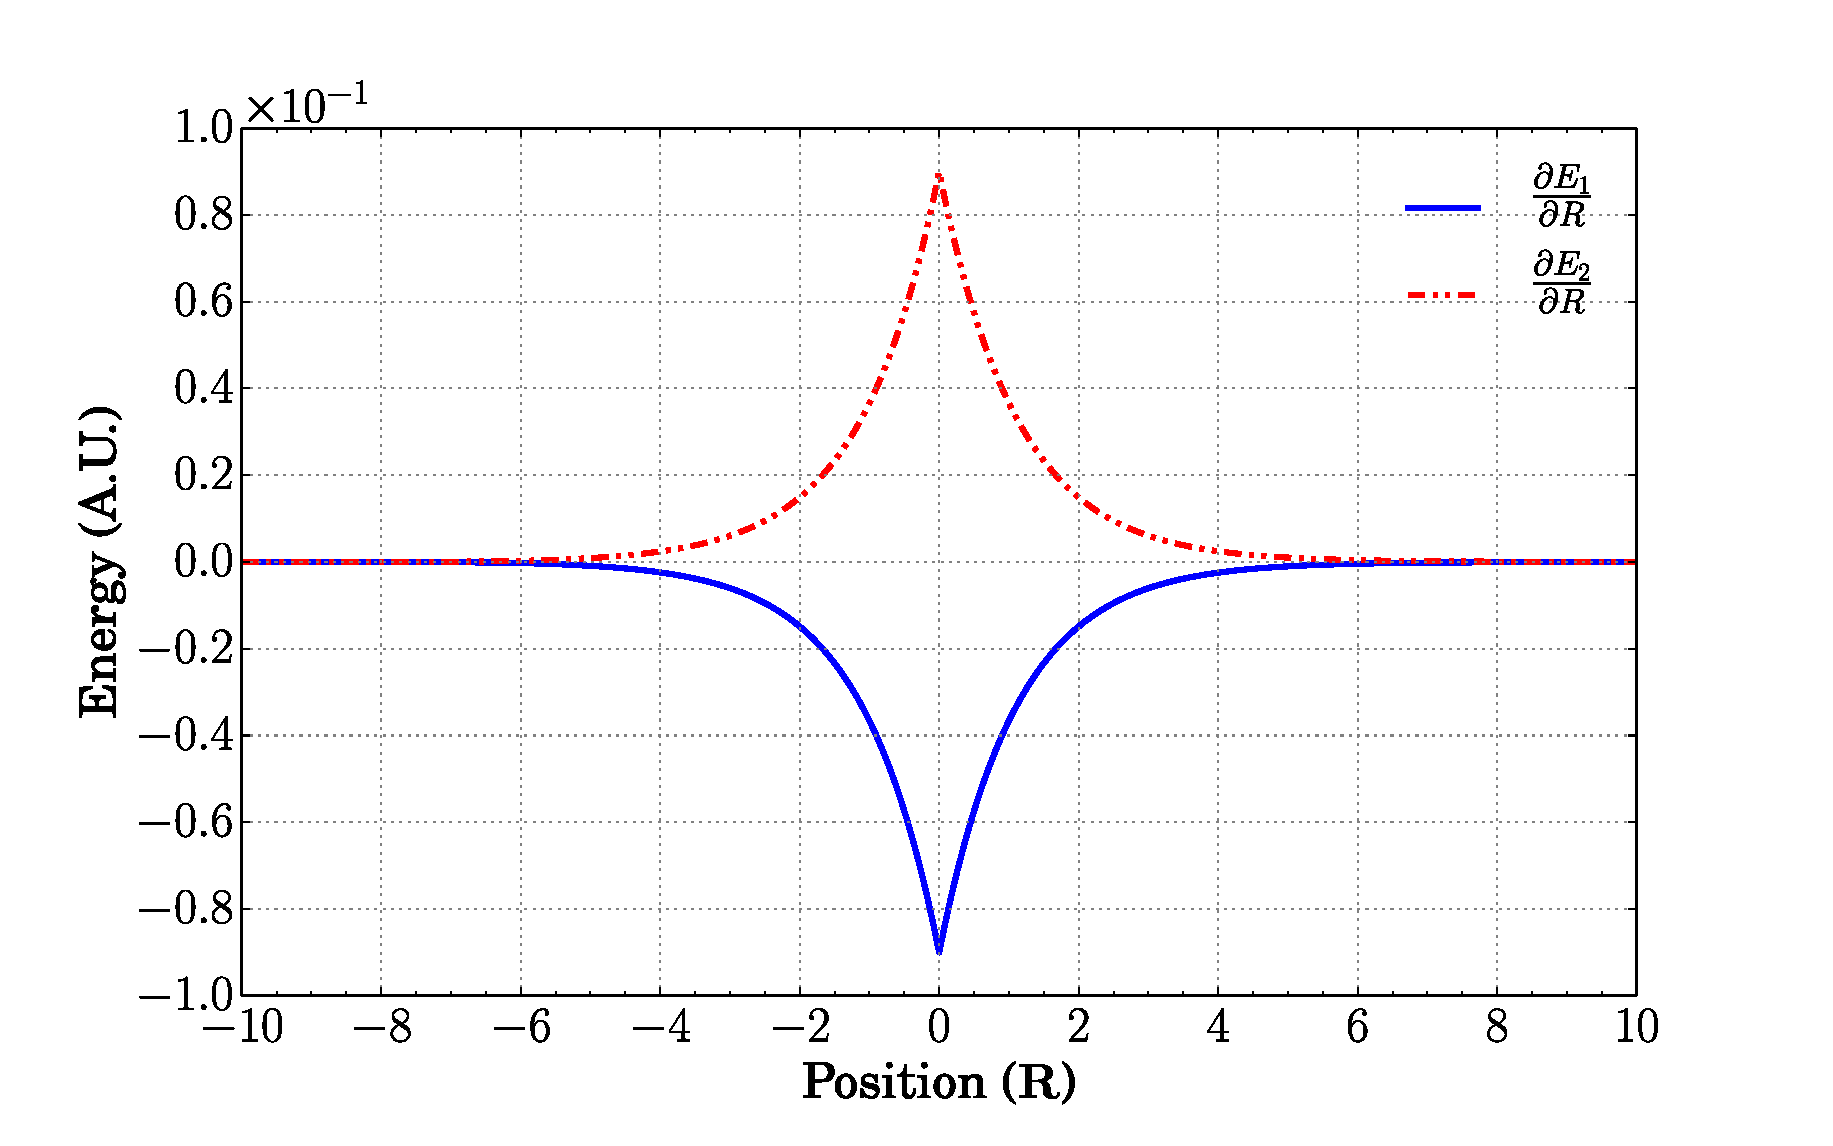
\includegraphics[scale=0.5]{daecpes.eps}
\caption[Extended coupling: adiabatic PES derivatives.]{Adiabatic PES derivatives. Derivatives of the eigenvalues of the diabatic Hamiltonian matrix.}
\label{f:dapesec}
\end{figure}

The energy difference between both adiabatic PES is shown in \cref{f:delapesec}.

\begin{figure}
\centering
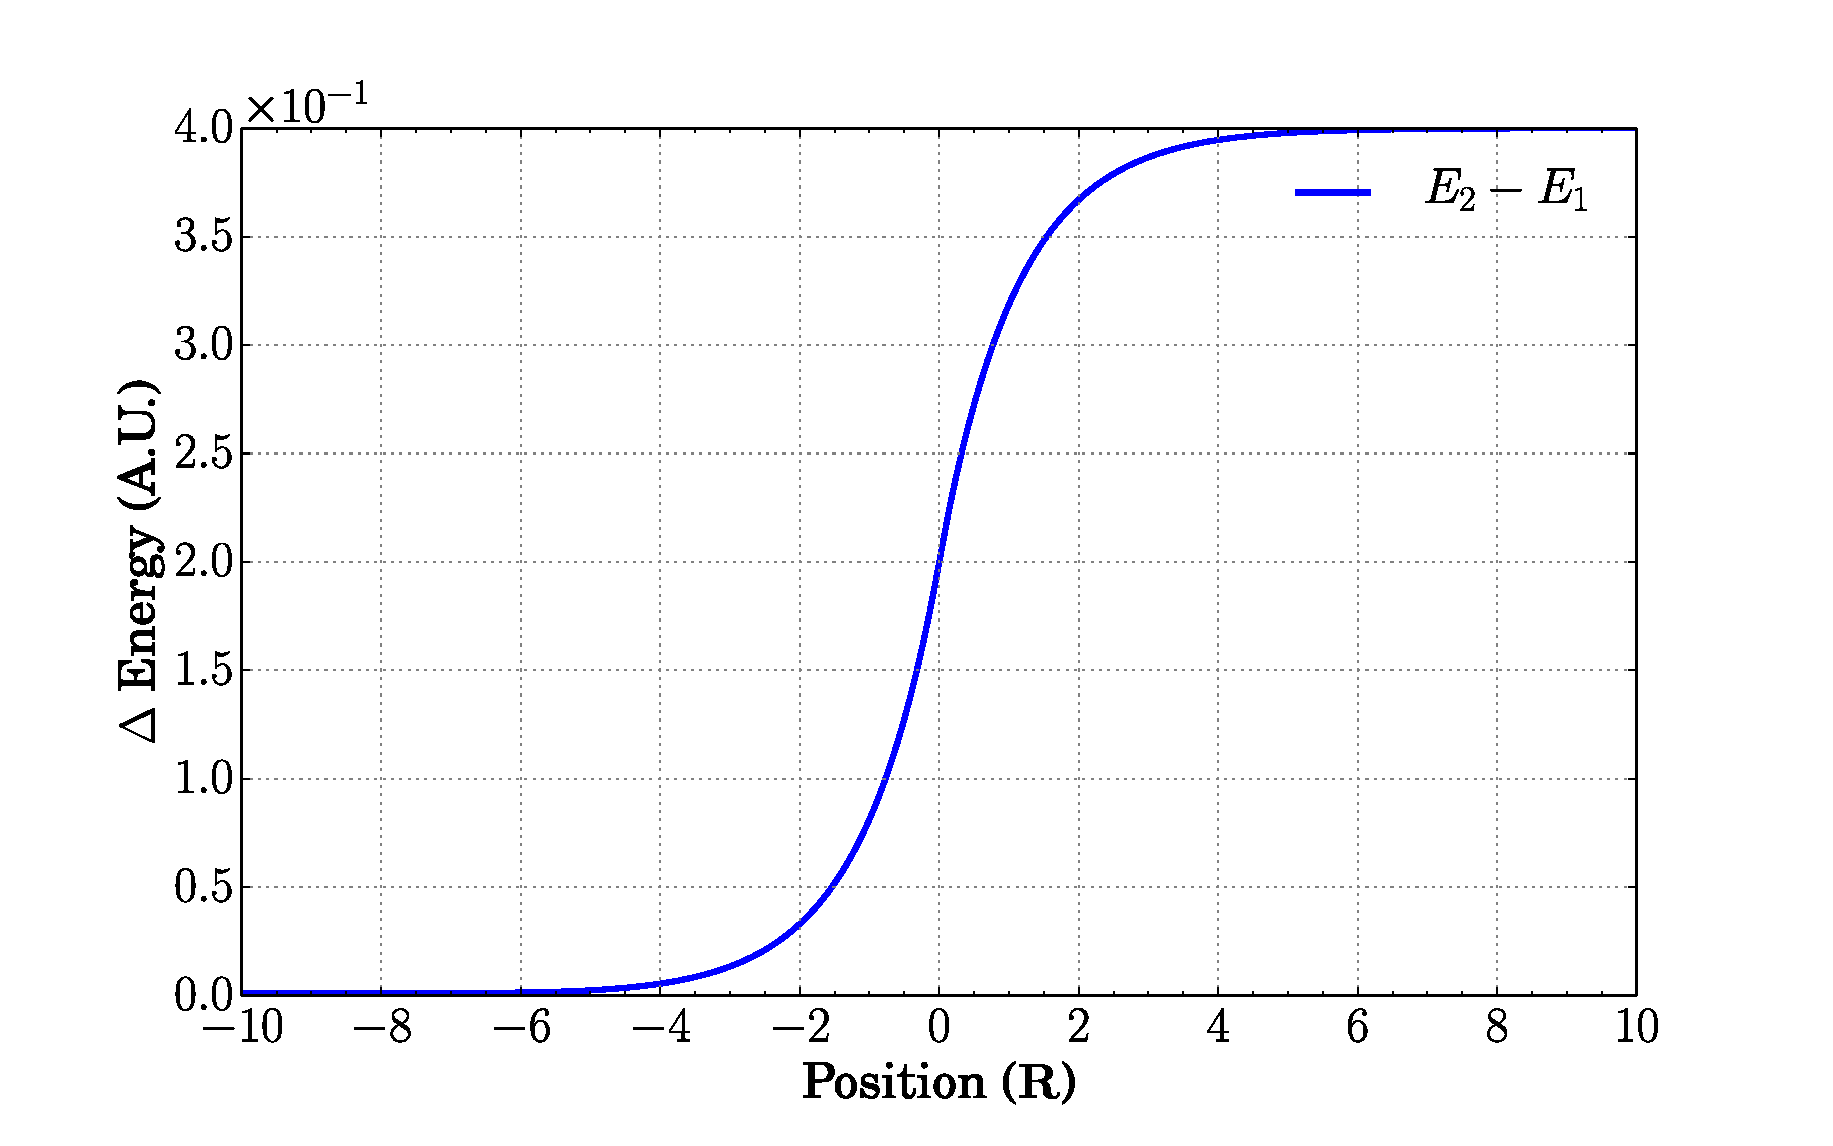
\includegraphics[scale=0.5]{del_aecpes.eps}
\caption[Extended coupling: energy difference between adiabatic PES]{Energy difference between adiabatic PES.}
\label{f:delapesec}
\end{figure}
%
\subsubsection{Equations of Motion}
%
The equations of motion are:
\begin{subequations}
\begin{align}
\dot{R} & = \frac{\chi}{\mu} \\
\dot{P} & = \frac{A B C}{2} \left(
\begin{cases}
e^{-C R} &\quad R\geq 0\\
e^{C R} &\quad R<0
\end{cases}
\right)
\left(\frac{(p_{1}^{2} + x_{1}^{2} - p_{2}^{2} - x_{2}^{2})\cdot \phi}{\eta} -\frac{(p_{2} x_{1} - p_{1} x_{2})\cdot \chi}{\mu \cdot \eta^{2}}
\right)\\
\dot{x_{1}} & = -\zeta\cdot x_{2} - \eta\cdot p_{1} \\
\dot{p_{1}} & = -\zeta\cdot p_{2} + \eta\cdot x_{1} \\
\dot{x_{2}} & = \zeta\cdot x_{1} + \eta\cdot p_{2} \\
\dot{p_{2}} & = \zeta\cdot p_{1} - \eta\cdot x_{2}~,
\end{align}
\end{subequations}
where,
\begin{subequations}
\begin{align}
&\phi = \frac{
B\begin{cases}
(2 - e^{-C R}) &\quad R \geq 0\\
e^{C R} &\quad R < 0
\end{cases}}{A} \\
&\eta = A\sqrt{1 + \phi^{2}}\\
&\chi = P + \frac{1}{2}(p_{2} x_{1} - p_{1} x_{2}) \arctan(\phi)\\
&\zeta =\frac{\arctan(\phi)\cdot \chi}{2 \mu}~.
\end{align}
\end{subequations}
%
\subsection{Spin-Boson Model for Condensed-Phase Dynamics}\label{sb:sb}
%
This problem is vastly different from the others. In our case, the model describes a 1D system of $ M $ coupled oscillators. More specifically, a one-dimensional lattice made up of $ M $ oscillating nuclei which posses bulk electronic states. What is measured here are not trajectories, but rather the time-dependent difference in the probability of finding the system in either of two electronic states; when the initial state $ =1 $, $ D(t) = P_{1\leftarrow 1} - P_{2\leftarrow 1}$, when the initial state $ =2 $, $ D(t) = P_{1\leftarrow 2} - P_{2\leftarrow 2}$.
%
\subsubsection{Potential Energy Surfaces}
%
The diabatic PES are defined as follows:
\begin{subequations}\label{eq:sbpes1}
\begin{align}
H_{11}(\bm{Q}) &= V_{0}(\bm{Q}) + V_{1}(\bm{Q}) + \epsilon \\
H_{22}(\bm{Q}) &= V_{0}(\bm{Q}) - V_{1}(\bm{Q}) - \epsilon \\
H_{12}(\bm{Q}) &= H_{12}(\bm{Q}) = \Delta~,
\end{align}
\end{subequations}
where,
\begin{subequations}\label{eq:sbpes2}
\begin{align}
V_{0}(\bm{Q}) &= \sum\limits_{k=1}^{M} \frac{1}{2} m_{k} \omega_{k}^{2} Q_{k}^{2} \\
V_{1}(\bm{Q}) &= \sum\limits_{k=1}^{M} c_{k} Q_{k}~.
\end{align}
\end{subequations}
For our purposes, the frequencies, $ \omega_{k} $, are uniformly distributed in the interval $ [0.01 \omega_{c},~4 \omega_{c}] $ \cite{spin-boson}, where $ \omega_{c} $ is known as the \emph{characteristic frequency}, and defines the system's overall time scale. The observant reader will realise this does not make a lot of sense on its own, because not all frequencies contribute to a system's energy in equal amounts. Which is why the coupling parameters, $ c_{k} $, are chosen so they obey the distribution:
\begin{align}\label{eq:sb_dd}
J(\omega) = \frac{\pi}{2} \sum\limits_{k=1}^{M} \frac{c_{k}^{2}}{m_{k} \omega_{k}}  \delta(\omega - \omega_{k})~,
\end{align}
where $ J(\omega) $ is an Ohmic distribution defined as:
\begin{align}\label{eq:sb_cd}
J(\omega) = \frac{\pi}{2} \alpha \omega \exp\left(-\frac{\omega}{\omega_{c}}\right)~,
\end{align}
where $ \alpha $ is the Kondo parameter (a coupling strength parameter). After equating \cref{eq:sb_dd,eq:sb_cd}, and integrating with respect to $ \omega $, we find the values of $ c_{k} $ to be:
\begin{subequations}
\begin{align}
c_{k} = \sqrt{\frac{2}{\pi} \Delta \omega m_{k} \omega_{k} J(\omega_{k})} 
&= \omega_{k} \sqrt{\alpha \Delta \omega m_{k} \exp\left(-\frac{\omega_{k}}{\omega_{c}}\right)} \\
\Delta \omega &= \frac{\omega_{max} - \omega_{min}}{M - 1}~.
\end{align}
\end{subequations}

The initial electronic conditions are initiated in the same manner as before. However, the nuclear ones are not. As stated before, the model describes oscillating nuclei in a 1D lattice, and their momenta and positions are assumed to follow the Wigner distribution:
\begin{subequations}
\begin{align}
\rho(\bm{P},\bm{Q}) &= \prod\limits_{k=1}^{M} \exp\left(-a_{k} \frac{P_{k}^{2}}{2 m_{k}}\right) \exp\left(-a_{k} \frac{1}{2} m_{k} \omega_{k}^{2} \left[Q_{k} + \frac{c_{k}}{m_{k} \omega_{k}^{2}}\right]^{2} \right)\\
a_{k} &= \frac{2}{\omega_{k}} \tanh\left(\frac{\beta \omega_{k}}{2}\right)~.
\end{align}
\end{subequations}
Which, in reality, is a bivariate normal distribution. Fortunately, the lack of a covariant term implies that positions and momenta can be independently sampled from normally distributed random numbers. In other words, the nuclei follow independent normal distributions for their momenta and positions. It is also worth noting that the argument for the total distribution is basically a scaled quasiclassical analogue of the quantum harmonic oscillator Hamiltonian operator ($ \hat{H} = \frac{\hat{p}^{2}}{2m} + \frac{1}{2} m \omega^{2} \hat{x}^{2}$), which makes a lot of intuitive sense, because it means the nuclear parameters are sampled according to the oscillators' normally distributed kinetic energy.

Sampling is done in the traditional way: assuming $ X $ is a normally distributed random number with unitary standard deviation and mean equal to zero, a normally distributed random number $ G $ with standard deviation equal to $ \sigma $ and mean equal to $ \mu $ can be calculated by $ G = \sigma X + \mu $. Given the definition of the normal distribution,
\begin{align}
G(x, \mu, \sigma) = \frac{1}{\sigma \sqrt{2\pi}} \exp\left[- \frac{(x-\mu)^{2}}{2 \sigma^{2}}\right]~,
\end{align}
the standard deviations and mean values of the nuclei's momenta and positions are:
\begin{subequations}
\begin{align}
&\sigma_{P_{k}} = \sqrt{\frac{m_{k} \omega_{k}}{2 \tanh\left(\frac{\beta \omega_{k}}{2}\right)}}\\
&\mu_{P_{k}} = 0\\
&\sigma_{Q_{k}} = \sqrt{\frac{1}{2 m_{k} \omega_{k} \tanh\left(\frac{\beta \omega_{k}}{2}\right)}}\\
&\mu_{Q_{k}} = -\frac{c_{k}}{m_{k} \omega_{k}^{2}}~.
\end{align}
\end{subequations}

The Gaussian sampling algorithm used, is a modified version of the Ziggurat algorithm originally written by George Marsaglia and Wai Wan Tsang\footnote{See \url{http://people.sc.fsu.edu/~jburkardt/f\_src/ziggurat/ziggurat.html}.}. The modification randomises the seed every time the subroutine is initialised, thus providing the accurate pseudo-random numbers necessary for reliable Monte Carlo simulations.
%
\subsubsection{Equations of Motion}
%
The equations of motion are obtained in exactly the same way as before (using the diabatic Hamiltonian), only we have defined $ M = 100 $ so there are 100 nuclear degrees of freedom (DOFs), which means there are 100 equations of motion for position and another 100 for momentum, giving a grand total of 204 equations. The nuclear equations of motion---as well as $ H_{11} $ and $ H_{22} $---are implemented as {\color{DarkViolet}\texttt{do}} loops:
\begin{subequations}
\begin{align}
\dot{Q_{j}} &= \frac{P_{j}}{m_{j}}\\
\dot{P_{j}} &= -m_{j}\omega_{j}^{2}Q_{j} - \frac{1}{2}c_{j}\cdot(p_{1}^{2} + x_{1}^{2} - p_{1}^{2} - x_{2}^{2})\\
\dot{x_{1}} & = p_{1}(V_{1} + \epsilon) + p_{2}\Delta\\
\dot{p_{1}} & = -x_{1}(V_{1} + \epsilon) - x_{2}\Delta\\
\dot{x_{2}} & = -p_{2}(V_{1} + \epsilon) + p_{1}\Delta\\
\dot{p_{2}} & = x_{2}(V_{1} + \epsilon) - x_{1}\Delta~.
\end{align}
\end{subequations}
%
\section{Code Structure}
%
\begin{itemize}
\item Main program.
\begin{enumerate}
\item Call data collection subroutine.
\item Call print PES and DPES subroutine.
\end{enumerate}
\item Data collection subroutine.
\begin{enumerate}
\item Declare and initialise variables.
\item Open output file.
\item Write heading on file.
\item Define value of initial momentum.
\item Call Monte-Carlo averaging routine.
\item Write final results.
\begin{itemize}
\item Repeat 4. to 6. for other initial momentum values.
\end{itemize}
\end{enumerate}
\end{itemize}

\begin{itemize}
\item Monte-Carlo averaging subroutine.
\begin{enumerate}
\item Declare and intialise variables.
\item Define Monte-Carlo steps loop.
\begin{enumerate}
\item Call solution subroutine.
\item Add results.
\end{enumerate}
\item Average results with the number of Monte-Carlo steps.
\item Calculate transition probabilities for reflection and transmission.
\end{enumerate}
\end{itemize}

\begin{itemize}
\item Solution subroutine.
\begin{enumerate}
\item Declare and initialise variables.
\item Define and calculate initial conditions and window functions.
\item Define integration loop.
\begin{enumerate}
\item Call RK4G subroutine using the appropriate equations of motion as argument.
\item Check for reflection, exit loop if the particle was reflected.
\item Update the initial conditions for next integration step.
\end{enumerate}
\item Calculate final values for the acceptance criteria.
\item Calculate final window functions.
\item Calculate results for the Monte-Carlo averaging subroutine.
\end{enumerate}
\end{itemize}

\begin{itemize}
\item Equations of motion subroutine.
\begin{enumerate}
\item Define and initialise variables.
\item Define equations of motion.
\end{enumerate}
\end{itemize}

\begin{itemize}
\item Runge-Kutta 4 Gill numerical integration routine (RK4G).
\begin{enumerate}
\item Define and initialise variables.
\item Call equations of motion subroutine.
\begin{itemize}
\item Calculate the intermediate step for all independent variables.
\end{itemize}
\item Repeat 2. for every intermediate step.
\item Calculate the final value of every independent variable, to be used in the next integration step.
\end{enumerate}
\end{itemize}

\begin{itemize}
\item PES and DPES printing subroutine.
\begin{enumerate}
\item Define and initialise variables.
\item Define loop to print all functions.
\begin{enumerate}
\item Open relevant output file.
\item Call PES and DPES subroutines.
\item Write numerical values of each PES and DPES function, evaluated at any given distance.
\begin{itemize}
\item Repeat b) and c) for all desired distances.
\end{itemize}
\end{enumerate}
\end{enumerate}
\end{itemize}

\begin{itemize}
\item PES or DPES subroutines.
\begin{enumerate}
\item Define and initialise variables.
\item Check which PES or DPES are required.
\item Define PES or DPES.
\end{enumerate}
\end{itemize}
%